% Twoside implica che i capitoli inizino sempre con la prima pagina a sinistra, eventualmente lasciando una pagina vuota nel capitolo precedente. 
\documentclass[a4paper, twoside,openright]{report}

% Dimensione dei margini
\usepackage[a4paper,top=3cm,bottom=3cm,left=3cm,right=3cm]{geometry} 
% Dimensione del font
\usepackage[fontsize=13pt]{scrextend}
% Lingua del testo
\usepackage[english,italian]{babel}
% Lingua per la bibliografia
\usepackage[fixlanguage]{babelbib}
% Codifica del testo
\usepackage[utf8]{inputenc} 
% Encoding del testo
\usepackage[T1]{fontenc}
% Per modificare l'header delle pagine 
\usepackage{fancyhdr}               

\usepackage{float}

% Librerie matematiche
\usepackage{amssymb}
\usepackage{amsmath}
\usepackage{amsthm}         

% Uso delle immagini
\usepackage{graphicx}
% Uso dei colori
\usepackage[dvipsnames, table]{xcolor}         
% Uso dei listing per il codice
\usepackage{listings}    
% Per andare a capo nei url
\usepackage[hyphens]{url}
% Per inserire gli hyperlinks tra i vari elementi del testo 
\usepackage{hyperref}     
% Diversi tipi di sottolineature
\usepackage[normalem]{ulem}

% -----------------------------------------------------------------

% Modifica lo stile dell'header
\pagestyle{fancy}
\fancyhf{}
\lhead{\rightmark}
\rhead{\textbf{\thepage}}
\fancyfoot{}
\setlength{\headheight}{16pt}

% Rimuove il numero di pagina all'inizio dei capitoli
\fancypagestyle{plain}{
  \fancyfoot{}
  \fancyhead{}
  \renewcommand{\headrulewidth}{0pt}
}

\definecolor{backcolour}{rgb}{0.90,0.95,0.92}

% Stile del codice
% \lstset{style=codeStyle}
\lstdefinestyle{codeStyle}{
    backgroundcolor=\color{backcolour},
    commentstyle=\color{teal},
    keywordstyle=\color{Magenta},
    numberstyle=\tiny\color{gray},
    stringstyle=\color{violet},
    basicstyle=\ttfamily\scriptsize,
    breakatwhitespace=false,     
    breaklines=true,                 
    captionpos=b,                    
    keepspaces=true,                 
    numbers=left,                    
    numbersep=5pt,                  
    showspaces=false,                
    showstringspaces=false,
    showtabs=false,
    tabsize=1
} \lstset{style=codeStyle}

% \lstset{style=longBlock}
\lstdefinestyle{longBlock}{
    commentstyle=\color{teal},
    keywordstyle=\color{Magenta},
    numberstyle=\tiny\color{gray},
    stringstyle=\color{violet},
    basicstyle=\ttfamily\scriptsize,
    breakatwhitespace=false,         
    breaklines=true,                 
    captionpos=b,                    
    keepspaces=true,                 
    numbers=left,                    
    numbersep=5pt,                  
    showspaces=false,                
    showstringspaces=false,
    showtabs=false,                  
    tabsize=2,
} \lstset{style=codeStyle}

% Togliendo il commento al comando che segue, si inseriscono nella bibliografia anche le fonti presenti in Bibliography.bib ma non citati direttamente con il comando \cite
\nocite{*}

% Margini prima e dopo blocchi di codice, per avere più distanza
\lstset{aboveskip=20pt,belowskip=20pt}

% Modifica dello stile dei riferimenti
\hypersetup{
    colorlinks,
    linkcolor=black,
    citecolor=black
}

% Aggiunti definizioni, teoremi, linea e listing
\newtheorem{definition}{Definizione}[section]
\newtheorem{theorem}{Teorema}[section]
\providecommand*\definitionautorefname{Definizione}
\providecommand*\theoremautorefname{Teorema}
\providecommand*{\listingautorefname}{Listing}
\providecommand*\lstnumberautorefname{Linea}

\raggedbottom



% -----------------------------------------------------------------
\begin{document}
\begin{titlepage}
\begin{figure}[!htb]
    \centering
\end{figure}
\vspace{30mm}
\begin{center}
    \LARGE{UNIVERSITÀ DEGLI STUDI DI MODENA E REGGIO EMILIA}
    \vspace{5mm}
    \\ \large{DIPARTIMENTO DI INGEGNERIA "ENZO FERRARI"}
    \vspace{5mm}
    \\ Laurea Triennale in Ingegneria Informatica
\end{center}

\vspace{15mm}
\begin{center}
    {\LARGE{\bf Augmented Reality Framework:\\ \vspace{5mm} AR Foundation }}
    
    % Se il titolo è abbastanza corto da stare su una riga, si può usare
    
    % {\LARGE{\bf Un fantastico titolo per la mia tesi!}}
\end{center}
\vspace{30mm}

\begin{minipage}[t]{0.47\textwidth}
	{\large{Relatore:}{\normalsize\vspace{3mm}
	\bf\\ \large{Prof: Nicola Bicocchi}}}
\end{minipage}

\hfill
\begin{minipage}[t]{0.47\textwidth}\raggedleft
	{\large{Candidato:}{\normalsize\vspace{3mm} \bf\\ \large{Manuel Gherardi}}}
\end{minipage}

\vspace{30mm}
\hrulefill
\\\centering{\large{Anno Accademico 2025/2026}}

\end{titlepage}
\let\cleardoublepage\clearpage
\include{chapters/Abstract}
\let\cleardoublepage\clearpage

\tableofcontents

\listoffigures

\chapter{Introduzione}
Negli ultimi anni, la Realtà Aumentata (AR) ha completato la sua transizione da tecnologia sperimentale a strumento pervasivo, capace di ridefinire l'interazione uomo-macchina in settori che spaziano dall'industria 4.0 alla medicina, fino all'istruzione e all'intrattenimento. A differenza della Realtà Virtuale, che isola l'utente in un ambiente digitale, l'AR arricchisce la percezione del mondo fisico sovrapponendovi elementi virtuali in tempo reale e in modo geometricamente coerente.Nonostante il potenziale rivoluzionario, la diffusione di massa delle applicazioni AR ha dovuto affrontare una barriera significativa: la frammentazione hardware e software. Per lungo tempo, lo sviluppo di soluzioni AR ha richiesto l'utilizzo di SDK(Software Development Kit) nativi differenti, come Apple ARKit per i dispositivi iOS e Google ARCore per l'ecosistema Android. Questa dicotomia ha storicamente comportato un aumento dei costi di produzione, problemi di portabilità del codice e una complessa gestione degli aggiornamenti.In questo panorama si colloca AR Foundation, il framework cross-platform sviluppato da Unity. AR Foundation si propone come uno strato di astrazione software che unifica le API dei principali sistemi operativi, permettendo agli sviluppatori di progettare un'architettura logica universale (“write once, run anywhere”). Attraverso l'uso di componenti modulari (come i Manager per il tracciamento delle superfici o dei volti), il framework non solo ottimizza il flusso di lavoro, ma garantisce l'accesso alle funzionalità hardware più avanzate dei dispositivi moderni senza perdere in prestazioni.
In questo lavoro, risultato dell'attivitá progettuale svolta presso il dipartimento di Ingegneria "Enzo Ferrari" dell'Universitá di Modena e Reggio Emilia, l'obiettivo è analizzare l'architettura e le potenzialità di AR Foundation come soluzione al problema della frammentazione nello sviluppo di applicazioni in Realtà Aumentata. Nella prima parte della tesi, a carattere compilativo, viene fornito un quadro comparativo dettagliato tra AR Foundation e gli SDK nativi sottostanti ARCore e ARKit, valutando l'impatto dell'astrazione in termini di funzionalità supportate, flessibilità architetturale e prestazioni. Successivamente, la trattazione si focalizzerà su una fase sperimentale, incentrata sulla progettazione e sull'implementazione di un'applicazione dimostrativa, al fine di quantificare sul campo l'efficienza del framework nei principali casi d'uso industriali o applicativi.
\chapter{Realtà Aumentata}

\section{Che cos’è la Realtà Aumentata?}

Per \textbf{realtà aumentata(AR, oppure Augmented Reality (RA))} \cite{augmented-reality-1}\cite{augmented-reality-2} si intende una tecnologia di computer grafica che integra in tempo reale informazioni digitali nell’ambiente reale dell’utente, arricchendone la percezione sensoriale con contenuti che i cinque sensi, da soli, non potrebbero cogliere. L’integrazione non comporta necessariamente un’aggiunta di informazioni: può consistere anche nella loro riduzione, quando ciò permette di rappresentare una situazione in modo più chiaro e utile. Gli elementi aumentati possono essere resi disponibili tramite dispositivi mobili come gli smartphone, tramite un PC dotato di webcam o di altri sensori, oppure tramite dispositivi indossabili di visione (ad es. occhiali a proiezione retinica), di ascolto (auricolari) e di manipolazione (guanti). \newline

Storicamente\cite{augmented-reality-3},le prime esperienze di realtà virtuale e aumentata risalgono agli anni ‘60. Nel 1962 Morton Heilig realizzò il Sensorama, una cabina che offriva un’esperienza multisensoriale con filmato stereoscopico, audio, vibrazioni, vento e odori, ma senza alcuna interattività. Nel 1968 Ivan Sutherland, il "padre della computer grafica", con il suo studente Bob Sproull, sviluppò il primo head-mounted display, noto come "Spada di Damocle", poichè era così pesante da dover essere sostenuto da un braccio meccanico attaccato al soffitto: mostrava grafiche wireframe tridimensionali, grazie a due tubi catodici, che seguivano i movimenti della testa, sovrapposte all’ambiente reale grazie a lenti semitrasparenti, e ne fanno quindi anche il primo sistema di AR. Il termine Augmented Reality fu coniato all’inizio degli anni '90 da Thomas Caudell e David Mizell, ricercatori della Boeing, che lo usarono per descrivere un display indossabile capace di sovrapporre al campo visivo dei tecnici le istruzioni digitali per il cablaggio degli aerei. Nel 1994 Paul Milgram e Fumio Kishino introdussero il continuum realtà-virtualità, che va dall’ambiente reale a quello completamente virtuale. Tra i due estremi si collocano l’Augmented Reality, prevalentemente reale con elementi virtuali aggiunti, e l’Augmented Virtuality, prevalentemente virtuale con elementi reali; l’intera fascia intermedia prende il nome di Mixed Reality. Infine, dalla metà degli anni 2010 si è diffuso il termine Extended Reality (XR), che non ha un singolo autore ma raggruppa VR, AR e MR.
Proprio in contemporanea all'AR, nel 1988 Mark Weiser \cite{ubiquitous-computing-1}\cite{ubiquitous-computing-2}\cite{ubiquitous-computing-3}, Chief Technologist presso il famoso centro di ricerca Xerox PARC(Palo Alto Research Center), formulò il concetto di \textbf{Ubiquitous Computing} (informatica ubiqua o pervasiva): una visione in cui i computer e le tecnologie associate diventano invisibili, fino a confondersi con la vita quotidiana. Questa invisibilità si realizza attraverso la "virtualità incarnata" (embodied virtuality), ovvero l’integrazione dei computer nel mondo fisico. Un’automobile moderna, ad esempio, può essere guidata in modo efficiente senza comprendere il funzionamento dei numerosi motori, attuatori e sensori che contiene: Weiser estese questa idea alle infrastrutture di calcolo e comunicazione, sintetizzandola così: \texttt{"Le tecnologie più profonde sono quelle che scompaiono. Si intrecciano nella trama della vita quotidiana fino a \newline diventarne indistinguibili"}\cite{ubiquitous-computing-3} \newline

L'AR si divide in due tipi\cite{The-virtuality-continuum}:
\begin{itemize}
    \item \textbf{Spatial AR}, Proietta la luce direttamente sull'ambiente reale (usando video proiettori fisici fissati nella stanza). Non richiede visori o smartphone per essere vista. Un esempio tipico è il spatial projection mapping (es. proiettare la trama di un tessuto su un divano reale). Consiste proprio nel proiettare interfacce o elementi digitali su superfici reali (tavoli, pareti, oggetti) e rendere quelle superfici interattive.

     \begin{figure}[H]
            \centering
            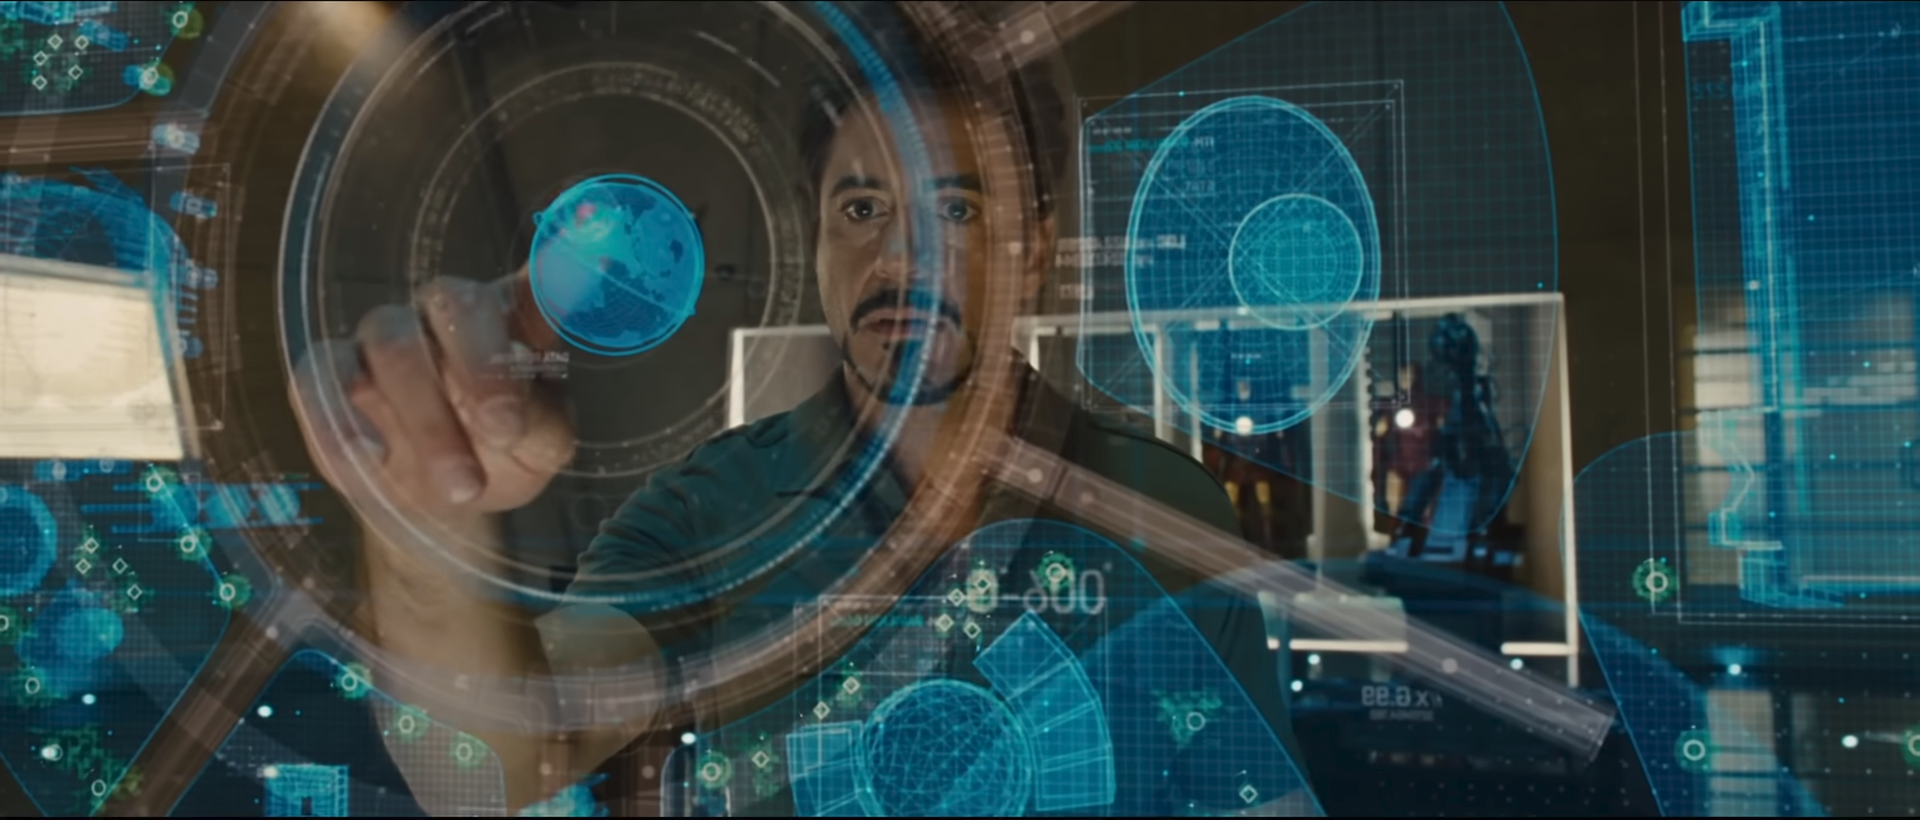
\includegraphics[width=0.7\textwidth]{images/augmented-reality/Spatial-AR.png} 
            \caption{Scene of Iron Man 2 (2010)\cite{img-ironman}}
            \label{fig:dt}
    \end{figure}

    
     \item \textbf{See-through AR}, in cui si fa uso di periferiche o dispositivi indossabili o di semplice visualizzazione come visore o schermi.

     \begin{itemize}
         \item \textbf{Optical See-through}, Vetri o lenti trasparenti (come i Google Glass o i Magic Leap) in cui la luce reale passa direttamente e le immagini digitali vengono proiettate sopra, quindi vedi il mondo reale direttamente con i tuoi occhi e la grafica vi viene sovrapposta tramite prismi/specchi.

        \begin{figure}[H]
            \centering
            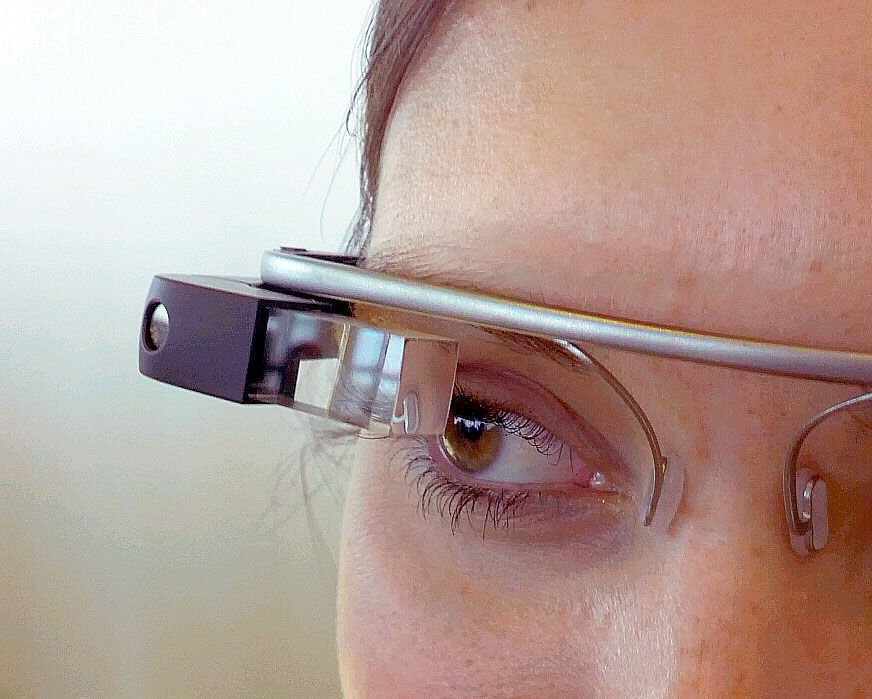
\includegraphics[width=0.6\textwidth]{images/augmented-reality/Google_Glass_detail.jpg} 
            \caption{Google Glass, 2013 \cite{img-google_glass}}
            \label{fig:dt}
        \end{figure}

         
         \item \textbf{Video See-through (Passthrough)}, che catturano il mondo reale tramite telecamere e lo riproiettano su schermi interni ad altissima risoluzione insieme agli elementi digitali. Visori chiusi (es. Apple Vision Pro, Meta Quest 3) o dispositivo con camera (es. Invizimals su PSP), dove microcamere riprendono l'esterno e mostrano il video su uno schermo insieme alla grafica 3D.

        \begin{figure}[H]
            \centering
            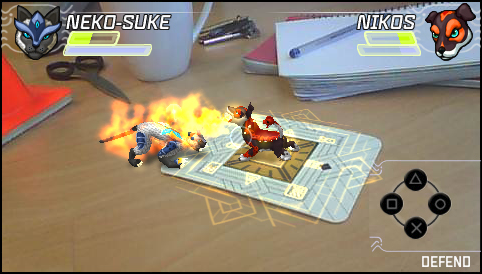
\includegraphics[width=0.7\textwidth]{images/augmented-reality/invizimals.png} 
            \caption{An example of AR videogame: Invizimals, game of PSP \cite{img-invizimals}}
            \label{fig:dt}
        \end{figure}
     \end{itemize}

\end{itemize}


Dalla definizione precedentemente scritta, si può dedurre che l'AR è adatta ad ogni ambito\cite{augmented-reality-1}: 

\begin{itemize}
    \item[-] \textbf{ Medicina e Sanità} \newline
    in medicina e sanità si introduce per migliorare la chirurgia assistita, ovvero tramite sovrapposizione di scansioni (TAC, risonanze) direttamente sul corpo del paziente durante gli interventi per guidare l'incisione e la precisione del chirurgo, e sempre in questo ambito, si usa per la formazione di medici mediante simulazioni delle procedure mediche e anatomiche su modelli virtuali interattivi senza rischi per i pazienti;

     \item[-] \textbf{ Industria e Luogo Lavorativo} \newline
    nell'industria e in ambito lavorativo in generale viene introdotta nella manutenzione e assemblaggio, mediante istruzioni di montaggio o schemi tecnici sovrapposti in tempo reale sui macchinari per guidare i tecnici a mani libere (remote assistance), e anche sulla sicurezza, in cui consiste nella segnalazione visiva di pericoli o aree ad alto rischio direttamente nel campo visivo degli operatori;

     \item[-] \textbf{ Architettura, Progettazione e Pianificazione Urbana} \newline
    in architettura, progettazione e pianificazione Urbana viene usata nella visualizzazione dei progetti, per il rendering 3D di edifici o strutture sovrapposti sul terreno reale prima dell'inizio dei lavori, oppure per l'ispezione di interni, offrendo la possibilità di guardare "attraverso le pareti" per individuare tubature, cablaggi o elementi strutturali interni;

     \item[-] \textbf{ Archeologia, Cultura e Turismo} \newline
    In archeologia, cultura e turismo viene impiegato nella ricostruzione di rovine, nella visualizzazione in tempo reale di come apparivano monumenti ed edifici antichi direttamente sopra i siti archeologici attuali, e nelle guide ed esperienze di musei, tramite punti di interesse interattivi e contenuti multimediali sovrapposti alle opere o alle attrazioni turistiche della città;

     \item[-] \textbf{Commercio, Marketing e Retail} \newline
    nel commercio, marketing e retail, con la famosa filosofia del "Try Before You Buy" (Prova prima di acquistare): con la visualizzazione di mobili e oggetti d'arredo nell'ambiente di casa prima dell'acquisto, oppure prova virtuale di capi d'abbigliamento, occhiali e cosmetici, e con l'Augmented Advertising, che consiste in campagne pubblicitarie interattive accessibili inquadrando imballaggi, riviste o cartelloni;

     \item[-] \textbf{ Istruzione e Formazione (STEM)} \newline
    nell'istruzione e formazione (STEM) tramite libri e materiali interattivi, ovvero con l'integrazione dei libri di testo classici con modelli 3D animati di molecole, organi o corpi celesti e in ambito più pratico con l'addestramento al volo e militare tramite display o visori per piloti (Head-Up Display o HUD) con dati tattici, rotte e parametri di volo sovrapposti al parabrezza;

     \item[-] \textbf{Automotive e Navigazione} \newline
    nell'automotive e navigazione sempre usando l'implementazione precedente, ovvero tramite Head-Up Display (HUD) proiettando i dati di navigazione, velocità e segnali stradali direttamente sul parabrezza dell'auto, e nella navigazione pedonale o per veicoli, tramite indicazioni stradali visive e frecce dinamiche sovrapposte direttamente sulla strada inquadrata dalla fotocamera;
     
     \item[-] \textbf{ Intrattenimento e Videogiochi} \newline
    nell'intrattenimento e nei videogiochi, in cui consiste nel gaming geolocalizzato, ovvero videogiochi che trasformano l'ambiente cittadino reale in un campo da gioco interattivo (es. Pokemon GO);

     \item[-] \textbf{ Eventi dal Vivo e Trasmissioni} \newline
    infine negli eventi dal vivo e trasmissioni, mediante grafiche e statistiche in tempo reale sovrapposte ai campi durante gli eventi sportivi.
\end{itemize}

\section{ Pro e Contro }
In tutti questi ambiti, possiamo studiare e analizzare come l'AR si comporta sotto diversi aspetti e stilare una lista di caratteristiche che può portare questa tecnologia, sia positive sia negative.

\subsection{Pro}

\begin{enumerate}
    \item \textbf{Continuità con la realtà e sicurezza d'uso} \newline
    A differenza della realtà virtuale (VR), che isola completamente l'utente portandolo in un mondo artificiale, la realtà aumentata mantiene la persona ancorata all'ambiente fisico reale. Questo offre vantaggi cruciali:
    \begin{itemize}
        \item \textbf{Consapevolezza dell'ambiente circostante} \newline
        L'utente continua a vedere dove cammina o lavora, riducendo rischi di collisione o disorientamento.
        \item \textbf{Minore affaticamento visivo/sensoriale} \newline
        Non dovendo ricreare un intero mondo 3D ma solo "strati" di informazione, l'esperienza risulta spesso più naturale e meno alienante.
    \end{itemize}

    \item \textbf{Miglioramento della precisione e riduzione degli errori umani} \newline
    La sovrapposizione visiva di dati e modelli direttamente sull'oggetto o sul corpo su cui si sta lavorando elimina la necessità di consultare continuamente manuali o schermi esterni:
    \begin{itemize}
        \item \textbf{Minori tassi di errore} \newline
        In ambiti critici come la chirurgia o la manutenzione industriale, le guide visive passo-passo riducono le dimenticanze e gli sbagli operativi.
        \item \textbf{Aumento della velocità di esecuzione} \newline
        L'operatore o il tecnico ha le mani libere e le informazioni visive posizionate esattamente dove servono.
    \end{itemize}

    \item \textbf{Abbattimento dei costi e ottimizzazione dei processi} \newline
    \begin{itemize}
        \item \textbf{Prototipazione e visualizzazione anticipata} \newline
        Architetti, designer e pianificatori possono testare un progetto nell'ambiente reale prima di costruire o produrre fisicamente il bene, riducendo lo spreco di materiali e correggendo difetti in anticipo.
        \item \textbf{Riduzione dei resi nel commercio} \newline
        La possibilità di provare virtualmente mobili o vestiti prima dell'acquisto ("Try Before You Buy") aumenta la certezza del consumatore e abbassa la quota di resi.
    \end{itemize}

    \item \textbf{Esperienza di apprendimento più intuitiva e coinvolgente} \newline
    \begin{itemize}
        \item \textbf{Apprendimento con l'esperienza} \newline
        Sia nell'istruzione scolastica (STEM) sia nella formazione aziendale, visualizzare ed interagire con oggetti 3D (come molecole, motori o organi anatomici) facilita la comprensione di concetti complessi rispetto alla sola lettura.
        \item \textbf{Accessibilità del sapere} \newline
        Le informazioni guida o storiche vengono erogate in modo contestuale (es. inquadrando un monumento o una rovina), rendendo l'esplorazione autonoma e ricca di valore culturale.
    \end{itemize}

    \item \textbf{Collaborazione e assistenza a distanza} \newline
    \begin{itemize}
        \item \textbf{Remote Assistance} \newline
        Esperti qualificati possono guidare tecnici o utenti sul campo disegnano indicazioni visive direttamente nello schermo di chi opera, eliminando tempi e costi di trasferta.
        \item \textbf{Lavoro di squadra facilitato} \newline
        Più persone possono visualizzare e manipolare simultaneamente lo stesso modello 3D nello spazio reale.
    \end{itemize}

\end{enumerate}


\subsection{Contro}

Nonostante i numerosi vantaggi, la diffusione della realtà aumentata comporta diversi rischi, pericoli e svantaggi che spaziano dalla sicurezza fisica alle implicazioni etiche e sociali.

\begin{enumerate}
    \item \textbf{Rischi per la sicurezza fisica e distrazione} \newline
    \begin{itemize}
        \item \textbf{Saturazione cognitiva e perdita di attenzione} \newline
        L'accumulo di informazioni visive sovrapposte al mondo reale può sovraccaricare il cervello, riducendo la prontezza di riflessi in situazioni critiche (come la guida di veicoli o la gestione di macchinari)
        \item \textbf{Incidenti da distrazione} \newline
        L'uso continuo di visori o smartphone per interagire con contenuti AR nell'ambiente urbano aumenta il rischio di cadute, attraversamenti involontari o collisioni con ostacoli e persone.
    \end{itemize}

     \item \textbf{Privacy e sorveglianza invasiva} \newline
    \begin{itemize}
        \item \textbf{Raccolta costante di dati ambientali e personali} \newline
        Per funzionare, i dispositivi AR utilizzano fotocamere e sensori sempre attivi che mappano continuamente l'ambiente circostante, registrando volti di passanti, targhe ed spazi privati senza consenso esplicito.
        \item \textbf{Tracciamento dei comportamenti e biometria} \newline
        I visori avanzati monitorano lo sguardo (eye tracking), i movimenti del corpo e le reazioni emotive, fornendo alle aziende dati estremamente sensibili sulle preferenze e sull'attenzione degli utenti.

    \end{itemize}

    \item \textbf{Sicurezza informatica e manipolazione della realtà} \newline
    \begin{itemize}
        \item \textbf{Hacking ed estorsione informativa} \newline
        Un attacco informatico potrebbe iniettare informazioni false nel campo visivo dell'utente (ad esempio alterare i segnali stradali su un display guida o nascondere un ostacolo reale), con conseguenze potenzialmente fatali, portando quindi a danni irreversibili o comunque molto gravi ad ambiente, beni o addirittura persone.

        \item \textbf{Falsificazione del contesto (Reality Hacking)} \newline
       Sovrapporre elementi grafici non autorizzati o ingannevoli su luoghi fisici (come pubblicità abusive, messaggi diffamatori o informazioni manipolate) può alterare la percezione della realtà da parte degli utenti.

    \end{itemize}

     \item \textbf{Impatto Psicologico e Dipendenza} \newline
     Rischi in comune con i Social Network:
    \begin{itemize}
        \item \textbf{Sovraccarico sensoriale e alienazione} \newline
        La costante sovrapposizione di notifiche e contenuti digitali al mondo fisico rende difficile la disconnessione, aumentando i livelli di stress e ansia.

        \item \textbf{} Un utilizzo incontrollato può portare a preferire l'ambiente arricchito dai filtri digitali rispetto al mondo reale, condizionando negativamente la socializzazione e le relazioni interpersonali dirette.


    \end{itemize}

    \item \textbf{Limiti Tecnici ed Economici} \newline
     
    \begin{itemize}
        \item \textbf{Costi elevati dei dispositivi} \newline
        I visori e gli strumenti AR di livello professionale mantengono prezzi accessibili solo a grandi aziende o settori specializzati, rischiando di ampliare il divario digitale (digital divide)

        \item \textbf{Consumo energetico e limiti hardware} \newline
        I sensori e i processori AR richiedono un'elevata potenza di calcolo, comportando una durata limitata della batteria e problemi di surriscaldamento nei dispositivi portatili.


    \end{itemize}

\end{enumerate}



\section{ Come funziona? }

\textbf{Architettura}
 \begin{figure}[H]
            \centering
            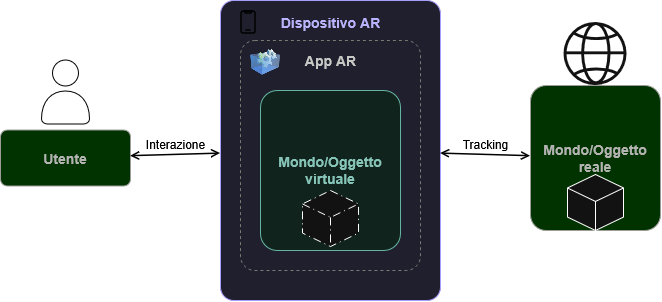
\includegraphics[width=0.8\textwidth]{images/augmented-reality/AR-Working-General-Architecture.png} 
            \caption{AR General Working Architecture\cite{img-ar-architecture}}
            \label{fig:dt}
\end{figure}

Il funzionamento di un sistema di AR si basa su un ciclo continuo di elaborazione (loop di feedback) suddiviso in tre fasi sequenziali fondamentali\cite{augmented-reality-2}:

\begin{figure}[H]
            \centering
            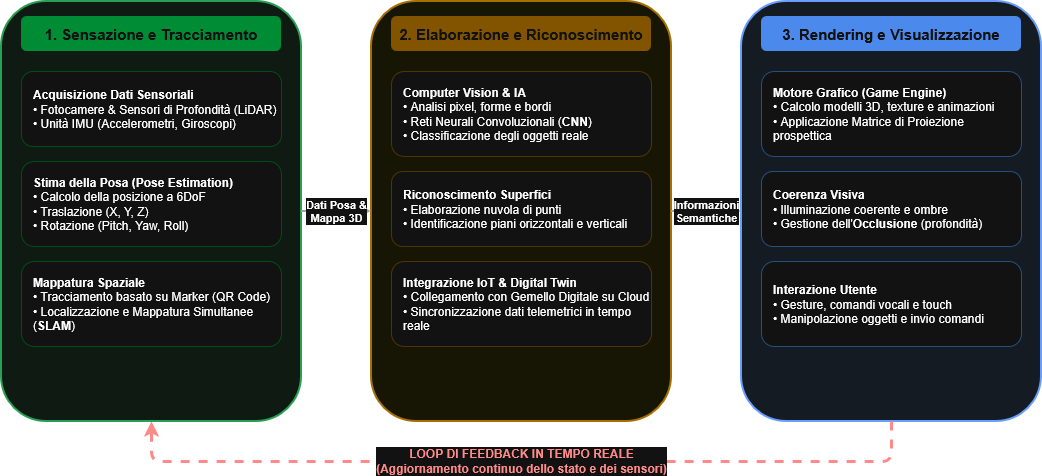
\includegraphics[width=1\textwidth]{images/augmented-reality/The-typical-pipeline-of-an-AR-application.png} 
            \caption{AR Pipeline}
            \label{fig:dt}
    \end{figure}

\begin{itemize}
    \item \textbf{Sensazione e Tracciamento} \newline
    Per fare in modo che gli elementi virtuali possano essere inseriti nel mondo reale in modo credibile, uno smartphone o un visore devono comprendere in tempo reale e con estrema precisione dove si trovano nello spazio tridimensionale. Per ottenere questo risultato, il dispositivo si affida all'acquisizione continua di flussi video e dati fisici attraverso una combinazione di sensori ottici e inerziali. Tra i sensori ottici troviamo le fotocamere tradizionali, che riprendono l'ambiente circostante, e i sensori di profondità avanzati come il LiDAR, che emettono impulsi di luce invisibile per calcolare la distanza esatta degli oggetti e creare una mappa tridimensionale millimetrica dello spazio. A questi si affiancano l'Unità di Misura Inerziale, comunemente nota come IMU, che integra accelerometri per misurare le variazioni di velocità e giroscopi per tracciare l'orientamento e la velocità di rotazione. Grazie a questa componentistica, il sistema è in grado di captare anche i movimenti minimi o rapidi della testa o delle mani dell'utente, compensando i ritardi visivi e garantendo la fluidità dell'esperienza. \newline

    L'aspetto più importante di questa fase è la cosiddetta stima della posa, o Pose Estimation, che calcola la posizione e l'orientamento del dispositivo in sei gradi di libertà, noti come 6DoF. Questi sei gradi descrivono tutte le possibili modalità di movimento di un corpo nello spazio: tre riguardano la traslazione lineare lungo gli assi cartesiani, ovvero lo spostamento in avanti e indietro, a sinistra e a destra, e in alto e basso; gli altri tre riguardano la rotazione, specificatamente l'inclinazione in avanti e indietro nota come pitch, la rotazione orizzontale a destra e sinistra nota come yaw, e l'inclinazione laterale nota come roll. Per calcolare questi dati e mappare l'ambiente, i dispositivi utilizzano principalmente due strade. La prima è il tracciamento basato su marcatori, o Marker-based, in cui il software riconosce simboli o pattern geometrici prestampati, come i codici QR; conoscendo le dimensioni e la posizione esatta del marcatore nel mondo reale, il sistema sa immediatamente dove posizionare il contenuto virtuale. La seconda tecnica, molto più avanzata e utilizzata negli ambienti aperti o non preparati, è la localizzazione e mappatura simultanee, nota come SLAM. Questa tecnologia consente al dispositivo di costruire progressivamente una mappa 3D dell'ambiente circostante e, nello stesso identico momento, di calcolare la propria posizione esatta all'interno di quella mappa senza bisogno di alcun punto di riferimento esterno, permettendo all'utente di muoversi liberamente.

    \begin{figure}[H]
            \centering
            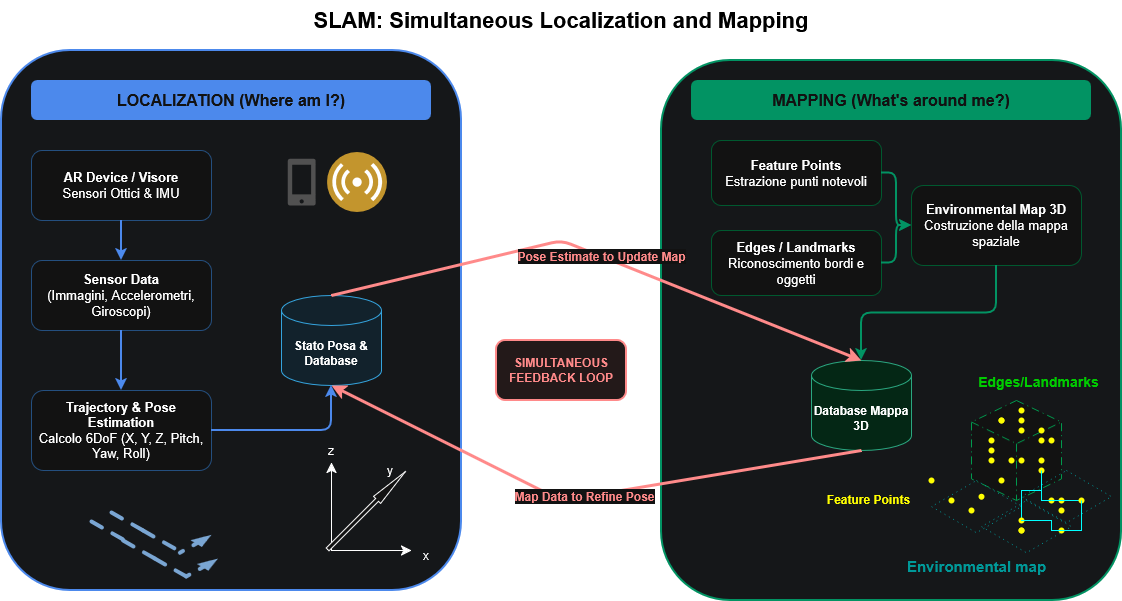
\includegraphics[width=1\textwidth]{images/augmented-reality/SLAM.png} 
            \caption{SLAM \cite{img-SLAM}}
            \label{fig:dt}
    \end{figure}

    \item \textbf{Elaborazione e Riconoscimento} \newline
    Una volta che i dati grezzi sono stati raccolti dai sensori e dalle fotocamere, il software li interpreta e cerca di dare un significato logico e semantico a ciò che la telecamera sta inquadrando. Questo processo si fonda sui principi della Computer Vision, ovvero la branca dell'intelligenza artificiale che permette ai computer di "vedere" e comprendere le immagini e i video digitali, analizzando i singoli pixel per riconoscere bordi, forme, angoli e variazioni di luce. Per fare un salto di qualità nell'interpretazione dell'ambiente, gli algoritmi si affidano a modelli di intelligenza artificiale complessi, come le reti neurali convoluzionali, note anche come CNN. Queste reti di apprendimento profondo sono particolarmente abili nell'elaborazione visiva e consentono al sistema di classificare gli oggetti con precisione, distinguendo ad esempio un tavolo da una sedia, una parete da una porta, oppure riconoscendo un componente meccanico specifico all'interno di un'officina.    \newline

    Attraverso questo processo, il software riesce a riconoscere i piani e le superfici fisiche presenti nell'ambiente, elaborando la nuvola di punti creata nella fase precedente per identificare le superfici orizzontali, come pavimenti e tavoli, e quelle verticali, come le pareti. Questa capacità è fondamentale perché permette agli oggetti virtuali di "posarsi" in modo logico sul mondo reale, come fare in modo che una sedia olografica poggi saldamente sul pavimento di una stanza. In contesti industriali o smart factories particolarmente avanzati, questa fase di riconoscimento si spinge oltre, prevedendo l'interconnessione con un Digital Twin, ovvero un gemello digitale memorizzato sul cloud. Quando il sistema inquadra un macchinario reale, non si limita a riconoscerne la forma geometrica nello spazio, ma lo associa alla sua controparte virtuale dinamica. Questo collegamento permette di sincronizzare in tempo reale i dati telemetrici, come la pressione, la temperatura e i cicli di lavoro, e lo stato di salute dell'impianto provenienti dai sensori IoT, ovvero gli oggetti intelligenti connessi a Internet, consentendo all'operatore di visualizzare grafici, schemi e avvisi diagnostici direttamente sovrapposti al macchinario che sta guardando.

    \item \textbf{Rendering e Visualizzazione} \newline
    Infine il software si occupa di generare concretamente l'immagine finale che l'utente vedrà attraverso lo schermo del dispositivo, fondendo in modo fluido, coerente e in tempo reale il mondo reale con quello virtuale. A occuparsi di questo compito è il motore grafico, o Game Engine, un software potente originariamente sviluppato per l'industria dei videogiochi ma oggi indispensabile in AR, che si incarica di calcolare la geometria dei modelli tridimensionali, applicare le texture, cioè i materiali visivi e i colori, gestire le animazioni e simulare le leggi della fisica sugli oggetti olografici. Per fare in modo che l'illusione ottica sia perfetta, il motore grafico applica una matrice di proiezione, ovvero un calcolo matematico basato sulla posizione esatta del visore rilevata nella prima fase di tracciamento. Questo calcolo deforma e scala gli oggetti 3D rispettando le regole della prospettiva umana, facendo in modo che gli elementi virtuali vicini appaiano più grandi e quelli lontani più piccoli. \newline

    La coerenza visiva viene mantenuta grazie a due elementi cruciali: l'illuminazione coerente e l'occlusione. Nel primo caso, il sistema analizza le fonti di luce presenti nell'ambiente reale e illumina di conseguenza l'oggetto virtuale, generando ombre realistiche che ne impediscono l'effetto "piatto" o posticcio. Nel secondo caso, l'occlusione risolve il problema della profondità gestendo le sovrapposizioni: se una persona passa la mano o un oggetto reale davanti a un ologramma, la mano deve coprire l'oggetto virtuale perché si trova più vicina agli occhi rispetto ad esso. Senza l'occlusione, l'ologramma rimarrebbe sempre visibile in primo piano, rovinando completamente il senso di immersione. Infine, il ciclo si completa gestendo l'interazione dell'utente: attraverso gesture, ossia i movimenti delle mani tracciati dalle telecamere, comandi vocali o input touch, l'utente può manipolare l'oggetto virtuale, spostandolo, ridimensionandolo o aprendolo, oppure può inviare comandi diretti che modificano lo stato del mondo reale o dei sistemi fisici connessi.


\end{itemize}


\section{Tipologie di Realtà Aumentata}
Ne esistono due tipi: AR a riconoscimento Marker,la quale è più economica e accessibile, e Markerless AR, la quale offre un coinvolgimento maggiore.

\subsection{AR a Riconoscimento Marker}
Con questa tipologia, affinchè avvenga l'implementazione dell'AR, è necessario un trigger fisico (Marker) nell'ambiente reale, ad esempio un codice QR, un'immagine o un altro marker di destinazione. Quando la fotocamera di un dispositivo rileva il marker, attiva la visualizzazione dell'esperienza AR associata. Poiché questo tipo di AR è accessibile in qualsiasi momento da una serie di dispositivi, è quello più flessibile.
\subsection{Markerless AR}
Con questa tipologia, invece, non c'è alcun bisogno di un trigger fisico, poichè si basa direttamente su sensori, GPS, accelerometri e fotocamere del dispositivo per mappare in tempo reale l'ambiente circostante dell'utente. Questo mapping avviene spesso grazie ad algoritmi e alla computer vision, i quali determinano dove posizionare i contenuti digitali, rendendo l'esperienza più spontanea e dinamica.
 
\section{AR vs VR vs XR vs MR vs Spatial Computing}
Ora vedremo la differenza tra queste tecnologie molto simili ma diverse tra loro\cite{ar-vs-other}\cite{The-virtuality-continuum}:

\begin{itemize}
    \item \textbf{Virtual Reality (VR)} \newline
    Permette la creazione e l'immersione in un ambiente virtuale 3D, consentendo all'utente di muoversi liberamente e di interagire con esso. È possibile grazie ad elaboratori e interfacce dedicate, come visori, guanti dati (\textit{wired gloves}), cybertute e piattaforme omnidirezionali. Viene utilizzata per simulazioni, videogiochi e addestramento; un esempio diffuso è la serie di visori Meta Quest.
    Esistono due tipi: 
    \begin{itemize}
        \item \textbf{Semi-Immersive VR}, nel quale i dispositivi VR rappresentano in modo preciso e reale una parte del punto di vista dell'utente
         \item \textbf{Immersive VR}, dove i dispositivi rappresentano l'intero punto di vista dell'utente. 
    \end{itemize}

    \item \textbf{Spatial Computing} \newline
    È il paradigma tecnologico che consente ai sistemi informatici di comprendere, mappare e interagire con lo spazio fisico 3D così come fanno gli esseri umani. Permette ai contenuti digitali di "vivere" nell'ambiente reale con persistenza spaziale (ad esempio, posizionare un quadro digitale su una parete reale e ritrovarlo esattamente nella stessa posizione al successivo utilizzo del visore). Lo Spatial Computing fornisce le basi tecnologiche necessarie per abilitare la Mixed Reality.
    
    \item \textbf{Mixed Reality (MR)} \newline
    Fonde il mondo fisico e gli oggetti digitali, permettendo un'interazione dinamica in tempo reale tra elementi reali e virtuali (ad esempio, una palla virtuale che rimbalza sul pavimento reale di una stanza), che sfrutta lo Spatial Computing. Un esempio di dispositivo MR avanzato è l'Apple Vision Pro.

    \begin{figure}[H]
        \centering
        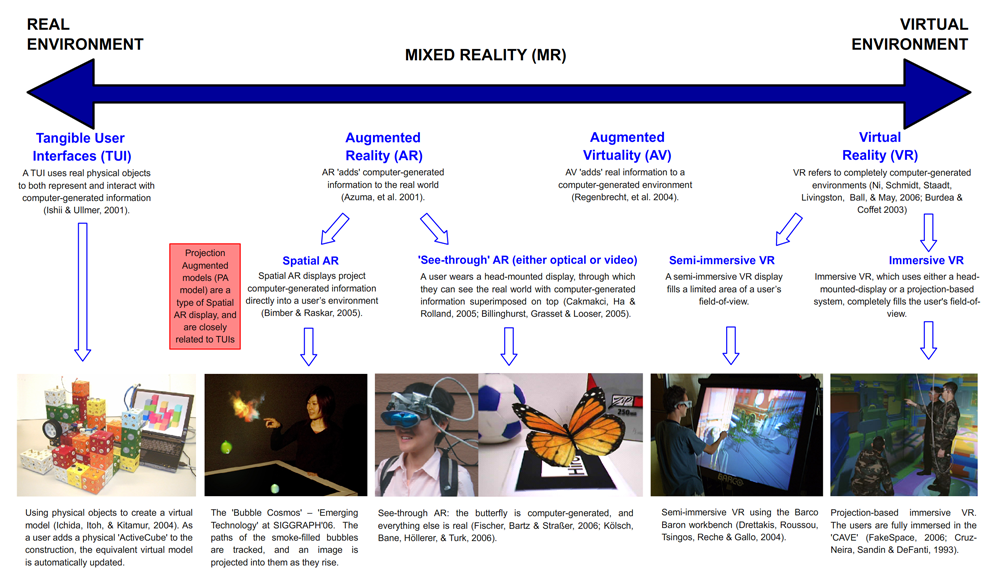
\includegraphics[width=0.7\textwidth]{images/augmented-reality/MR.png} 
        \caption{The Reality-Virtuality Continuum according to Milgram \cite{The-virtuality-continuum}}
        \label{fig:dt}
    \end{figure}

     dove AV è Augmented Virtuality, una tecnologia di MR in cui l'ambiente generato al computer viene arricchito da oggetti del mondo fisico. 
    
    \item \textbf{Extended Reality (XR)} \newline
    Termine che racchiude VR, AR e MR. Quando un dispositivo viene definito XR (come Apple Vision Pro o Galaxy XR), significa che è in grado di passare fluidamente tra diverse modalità di realtà immersiva. 
    
    In questo ambito rientra anche la \textbf{Augmented Reality (AR)} come detto in precedenza: l'integrazione in tempo reale di informazioni digitali nell'ambiente reale dell'utente, percepibili tramite dispositivi come smartphone, visori o auricolari. Tale integrazione può operare sia per addizione di elementi multimediali, sia per sottrazione di informazioni superflue (diminuzione della realtà), al fine di rendere la percezione dell'ambiente più chiara e funzionale.
    
\end{itemize}



\chapter{Unity}
Unity è un motore di gioco (\textit{game engine})\cite{Unity-1}\cite{Unity-2}\cite{Unity-3} multipiattaforma che consente lo sviluppo di videogiochi e altri contenuti interattivi, come visualizzazioni architettoniche o animazioni 3D in tempo reale. In questo capitolo introduco i concetti di Unity su cui si basa AR Foundation, necessari per comprendere il funzionamento dell'intero sistema.

\section{Pilastri di Unity}
Unity si basa su tre concetti. Il \textbf{GameObject} è l'entità di base della scena (un oggetto 3D, una luce, la camera): di per sé è un contenitore vuoto, il cui comportamento è definito dai \textit{componenti} associati. Il \textbf{Transform} è il componente presente in ogni GameObject e gestisce posizione (x, y, z), rotazione e scala nello spazio 3D della scena. I \textbf{MonoBehaviour} sono gli script C\# che si agganciano a un GameObject come componenti; ne fanno parte anche quelli di AR Foundation, come \texttt{ARPlaneManager} e \texttt{ARTrackedImageManager}. Questi script sfruttano i metodi del ciclo di vita di Unity (\texttt{Awake()}, \texttt{OnEnable()}, \texttt{Update()}, \texttt{OnDisable()}), richiamati automaticamente dal motore, ad esempio per aggiornare a ogni fotogramma gli oggetti 3D in base al movimento dello smartphone.

\section{Camera}
In un progetto senza AR la Camera è l'occhio del giocatore nello spazio virtuale. In AR svolge invece un doppio compito:

\begin{itemize}
    \item \textbf{Movimento}: la camera virtuale deve muoversi nella scena 3D esattamente come il telefono si muove nella stanza reale. Il componente \texttt{ARPoseDriver} aggiorna il Transform della Main Camera con la posa (posizione e rotazione) stimata dallo SLAM (\textit{Simultaneous Localization and Mapping}), ovvero la stima simultanea della posizione del dispositivo e della mappa dell'ambiente circostante.
    \item \textbf{Sfondo}: normalmente lo sfondo è un colore pieno o un cielo (\textit{Skybox}). Tramite \texttt{ARCameraBackground}, AR Foundation lo sostituisce con il flusso video in tempo reale della fotocamera del telefono.
\end{itemize}

\section{Sistema di coordinate}
Unity usa uno spazio di coordinate cartesiane 3D con origine in $(0,0,0)$, in cui per convenzione un'unità corrisponde a un metro. ARCore e ARKit creano invece un proprio sistema di coordinate (\textit{session space}), la cui origine coincide con la posizione del dispositivo all'avvio della sessione. In Unity, quando un GameObject è posto dentro un altro (relazione padre-figlio), le coordinate del figlio sono relative al padre. AR Foundation sfrutta questo meccanismo con un oggetto padre della camera (\texttt{XR Origin}), che converte il session space nel sistema di coordinate del mondo di Unity.

\section{Prefab e istanziazione}
Un \textit{Prefab} è un oggetto salvato come risorsa riutilizzabile, da cui Unity crea copie (istanze) a runtime con la funzione \texttt{Instantiate()}. Quando il telefono rileva un piano fisico (un tavolo, un pavimento), AR Foundation non disegna la geometria dal nulla: \texttt{ARPlaneManager} istanzia il prefab assegnato per ogni piano rilevato, aggiornandolo o rimuovendolo al variare del rilevamento. Lo stesso vale per ancore e altri \textit{trackable}. Lo sviluppatore usa invece \texttt{Instantiate()} per posizionare nella scena i propri contenuti virtuali.

\section{Raycasting}
Per capire ``dove tocca il dito sullo schermo nel mondo reale'' si usa il \textit{raycasting}, cioè il lancio di un raggio invisibile dalla camera attraverso un punto dello schermo, per trovare ciò che incontra lungo il suo percorso:

\begin{itemize}
    \item \textbf{Physics.Raycast}: è il raycasting standard di Unity. Il raggio (ottenibile con \texttt{Camera.ScreenPointToRay}) è testato contro i collider degli oggetti virtuali e restituisce il primo oggetto colpito.
    \item \textbf{ARRaycastManager}: applica lo stesso concetto, ma non usa il motore fisico di Unity: il raggio è testato contro i piani e i punti caratteristici (\textit{feature point}) rilevati dal sistema AR. Il metodo \texttt{Raycast} restituisce una lista di \texttt{ARRaycastHit} ordinata per distanza, ciascuno con una \texttt{pose} (posizione e rotazione del punto colpito); il tipo di superfici considerate si sceglie con \texttt{TrackableType}.
\end{itemize}

La posa restituita da \texttt{ARRaycastManager} viene tipicamente usata per istanziare un prefab sulla superficie toccata dall'utente.
\chapter{AR Foundation}
\textbf{AR Foundation}\cite{AR-Foundation-1}\cite{AR-Foundation-2} è un package di Unity (il game engine su cui è sviluppata l'applicazione; un \textit{package} è un insieme di codice e risorse che si aggiunge a un progetto Unity) che espone un'unica API (Application Programming Interface, cioè l'insieme di classi e funzioni che lo sviluppatore può richiamare) per le funzionalità di realtà aumentata, come il tracciamento della posizione della camera, il rilevamento dei piani, i raycast e le ancore. È quindi un framework \textit{cross-platform}, ovvero un insieme di strumenti e librerie che permette di scrivere il codice una sola volta e ottenere app per più sistemi operativi, in questo caso Android e iOS (oltre ad alcuni visori AR/XR), senza modifiche al codice. AR Foundation, però, definisce soltanto \textit{che cosa} si può chiedere al sistema e non contiene l'implementazione di \textit{come} farlo. Per questo si comporta da regista: Unity organizza le funzionalità AR in \textit{subsystem} XR, interfacce generiche come quella dei piani, della camera o dei raycast, e il compito di realizzarle concretamente spetta ai \textbf{plug-in provider}, package separati da installare e abilitare per ciascuna piattaforma di destinazione: \textbf{ARCore XR Plugin} per Android e \textbf{ARKit XR Plugin} per iOS. Ogni plug-in implementa i subsystem di Unity e fa da traduttore, convertendo le richieste generiche di AR Foundation nelle chiamate dello SDK nativo della piattaforma. Uno \textit{SDK} (Software Development Kit) è un insieme di librerie, strumenti e documentazione fornito dal produttore di una tecnologia: su Android è l'\textbf{ARCore SDK} di Google, mentre su iOS è il framework \textbf{ARKit} di Apple. Il plug-in appartiene quindi a Unity, lo SDK a Google o Apple, e lo sviluppatore scrive codice solo con l'API di AR Foundation. Le funzioni specifiche di ARCore, come Geospatial e Cloud Anchors, richiedono invece un package a parte, \textbf{ARCore Extensions}.

Il plug-in di ARCore usa la versione dello SDK che espone un'API in C (\textit{ARCore SDK for Android NDK}, libreria \texttt{libarcore\_sdk\_c.so}) ed è per questo che entra in gioco l'\textbf{NDK}\cite{NDK} (Native Development Kit), l'insieme di strumenti con cui Google permette di compilare per Android codice nativo, cioè codice C/C++ tradotto direttamente in istruzioni eseguibili dal processore del telefono. Il codice Java o Kotlin, invece, viene compilato in \textit{bytecode DEX} (un formato intermedio indipendente dal processore) ed eseguito da ART (Android Runtime), la macchina virtuale di Android; il codice nativo, non passando da questo livello, è in genere più veloce e permette di riutilizzare librerie C/C++ già esistenti, per cui viene preferito per le parti più critiche come la visione artificiale. Il risultato della compilazione nativa sono le \textit{shared library}, file con estensione \texttt{.so} (shared object) che il sistema carica in memoria solo a runtime, cioè quando l'app è in esecuzione. Poiché ogni architettura di processore (ABI, ad esempio \texttt{arm64-v8a}) richiede la propria versione compilata, le librerie vengono collocate in cartelle separate per ABI. Lo stesso meccanismo riguarda Unity stesso: con lo scripting backend \textbf{IL2CPP}, il codice C\# dell'app viene convertito in C++ e compilato con l'NDK in una libreria \texttt{.so}; le librerie del plug-in e dello SDK ARCore, invece, sono distribuite già compilate, per cui nella build l'NDK serve soprattutto a IL2CPP. Durante la fase di \textit{build}, la compilazione e il confezionamento del progetto, tutte queste librerie (quelle di Unity, quelle del plug-in e quelle dello SDK ARCore) vengono inserite nell'\textbf{APK} (Android Package Kit), il file di installazione di un'app Android, un archivio che contiene codice, risorse e manifest (per la pubblicazione su Google Play si usa invece l'\textbf{AAB}, Android App Bundle, da cui lo store ricava gli APK). Su iOS non esistono né NDK né file \texttt{.so}: il codice nativo viene compilato con Xcode in librerie statiche o framework.

Una volta installata l'app, il funzionamento a runtime segue una catena di chiamate che scende di livello a ogni passaggio. Quando uno script C\# invoca, ad esempio, \texttt{ARRaycastManager.Raycast} per capire quale superficie reale si trova sotto il punto toccato sullo schermo, AR Foundation inoltra la richiesta al subsystem corrispondente. Il provider di ARCore XR Plugin la raccoglie e, poiché il suo codice nativo è in C/C++, passa dal C\# alle funzioni delle librerie \texttt{.so} tramite \textit{P/Invoke} (Platform Invoke), il meccanismo di .NET per chiamare funzioni native. Queste librerie richiamano a loro volta l'API C dello SDK ARCore. Per le parti che invece vivono nel mondo Java, come la verifica dell'installazione di Google Play Services for AR o la richiesta dei permessi, si usa la \textbf{JNI} (Java Native Interface), il ponte che permette al codice nativo e a quello Java/Kotlin di chiamarsi a vicenda (in Unity spesso tramite \texttt{AndroidJavaObject}). Lo SDK, infine, non esegue da solo il tracciamento: comunica con il vero motore AR di sistema, \textbf{Google Play Services for AR}, un servizio separato dall'app che si installa e si aggiorna tramite Play Store, il quale analizza i frame della fotocamera e i dati dei sensori inerziali (accelerometro e giroscopio) per stimare la posizione del dispositivo e individuare i piani. Su iOS questo ruolo è svolto da ARKit, già integrato nel sistema operativo e quindi privo di installazione separata, dato che si aggiorna con iOS. I risultati compiono poi il percorso inverso: il motore AR restituisce i dati allo SDK, il plug-in li converte nelle strutture generiche dei subsystem e AR Foundation li espone allo sviluppatore, ad esempio sotto forma di oggetti \texttt{ARPlane}, aggiunti, aggiornati o rimossi man mano che il sistema rileva o affina i piani (evento \texttt{planesChanged}), permettendo di posizionare i contenuti virtuali sulla scena reale.



 \begin{center}
  Una lista di tutte le funzionalità che AR Foundation supporta:

    \begin{tabular}{| l | p{10cm} |}
      \hline
      \rowcolor{gray!30}
      \textbf{Caratteristica} & \textbf{Descrizione} \\ 
      \hline
      Sesssion & Attivare, disattivare e configurare la realtà aumentata sulla piattaforma di destinazione. \\ 
      \hline
      Device tracking & Tracciare la posizione e la rotazione del dispositivo nello spazio fisico. \\ 
      \hline
      Camera & Esegui il rendering delle immagini provenienti dalle fotocamere del dispositivo ed effettua la stima della luce \\ 
      \hline
      Plane Detection & Rileva e traccia le superfici piane. \\ 
      \hline
      Bounding Box Detection & Rileva e traccia i riquadri di delimitazione degli oggetti 3D. \\ 
      \hline
      Image Tracking & Rileva e traccia immagini 2D.\\ 
      \hline
      Markers & Traccia i marcatori AR e leggi i dati codificati in essi.\\ 
      \hline
      Object Tracking & Rileva e traccia oggetti 3D. \\ 
      \hline
      Face Tracking & Rilevare e tracciare i volti umani. \\ 
      \hline
      Body Tracking & Individuare e tracciare un corpo umano.\\ 
      \hline
      Point Clouds & Individua e traccia i punti caratteristici. \\ 
      \hline
      Ray Casts & Proietta raggi contro gli oggetti tracciati. \\
     \hline
      Anchors & Tracciare punti arbitrari nello spazio. \\
      \hline
      Meshing & Genera le mesh dell'ambiente.\\
      \hline
      Enviroment Probes & Genera mappe cubiche dell'ambiente. \\
      \hline
      Occlusion & Occulta i contenuti AR con oggetti fisici ed esegui la segmentazione umana. \\
      \hline
      Participants & Traccia altri dispositivi in una sessione AR condivisa. \\
      \hline
    \end{tabular}
\end{center}


\begin{center}
Non tutte le funzionalità sono supportate da tutte le piattaforme(Plug-in di Unity):

\begin{tabular}{| l | p{2cm} | p{2cm} |p{2cm} |}
      \hline
      \rowcolor{gray!30}
      \textbf{Caratteristica} & \textbf{Android} & \textbf{iOS} & \textbf{XR Sim.} \\ 
      \hline
      Sesssion & Si & Si & Si\\ 
      \hline
      Device tracking & Si & Si & Si \\ 
      \hline
      Camera & Si & Si & Si \\ 
      \hline
      Plane Detection & Si & Si & Si \\ 
      \hline
      Bounding Box Detection & & Si & Si\\ 
      \hline
      Image Tracking & Si & Si & Si\\ 
      \hline
      Markers &  & & \\ 
      \hline
      Object Tracking & & Si & \\ 
      \hline
      Face Tracking & Si & Si &\\ 
      \hline
      Body Tracking & & Si & \\ 
      \hline
      Point Clouds & Si & Si & Si\\ 
      \hline
      Ray Casts & Si & Si & Si \\
     \hline
      Anchors & Si & Si & Si \\
      \hline
      Meshing &  & Si & Si\\
      \hline
      Enviroment Probes & Si & Si & Si\\
      \hline
      Occlusion & Si & Si & Si\\
      \hline
      Participants &  & Si & \\
      \hline
    \end{tabular}
\end{center}

 \subsection{Architettura}
 
L'architettura di Unity AR Foundation \cite{AR-Foundation-1} si basa su tre concetti fondamentali, pensati per astrarre le differenze tra gli SDK nativi di realtà aumentata: \textbf{Subsystems}, \textbf{Managers} ed \textbf{Extensions}. 

 \begin{figure}[H]
            \centering
            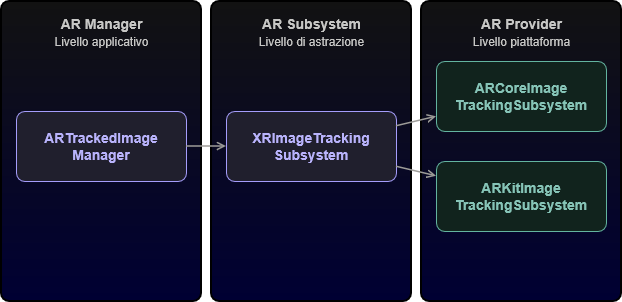
\includegraphics[width=0.8\textwidth]{images/ar-foundation/AR-Working.png} 
            \caption{AR Foundation Workflow (Example Feature: Image Tracking) \cite{AR-Foundation-3}}
            \label{fig:dt}
    \end{figure}

La figura mostra come collaborano i diversi livelli per una funzionalità di esempio, il tracciamento di immagini.
Al livello più alto si trova \texttt{ARTrackedImageManager}, un componente (\texttt{MonoBehaviour}) che lo sviluppatore aggiunge al GameObject \texttt{XR Origin} della scena. Serve a gestire gli eventi e ad accedere alle immagini tracciate, e permette di assegnare una \textit{Reference Image Library} (la lista di immagini da riconoscere) e un \textit{Prefab} da istanziare sopra l'immagine quando viene rilevata.
Al livello intermedio si trova \texttt{XRImageTrackingSubsystem}, il sottosistema che definisce l'interfaccia standard di Unity per il tracciamento di immagini, indipendente dal dispositivo. Stabilisce le regole e i metodi che ogni piattaforma (Android, iOS, ecc.) deve implementare, garantendo così il principio cross-platform.
Al livello più basso si trova il provider specifico della piattaforma, ovvero l'implementazione concreta fornita dal plug-in: ARCore XR Plugin su Android, ARKit XR Plugin su iOS. Il provider traduce i comandi generici del sottosistema in chiamate allo SDK nativo, che comunica con gli algoritmi di visione artificiale di ARCore per riconoscere, attraverso la fotocamera, i punti caratteristici (\textit{feature points}) dell'immagine di riferimento. Quando l'app viene compilata per Android, Unity attiva automaticamente il provider corrispondente.

\subsubsection{Subsystems}
Un \textbf{sottosistema}, implementato in Unity tramite la classe base \texttt{SubsystemWithProvider} \cite{AR-Foundation-1}, definisce il ciclo di vita e l'interfaccia di scripting di una specifica funzionalità del motore. Ad esempio, \texttt{XRPlaneSubsystem} definisce l'interfaccia di tracciamento dei piani: lo stesso codice applicativo può usare un piano rilevato sia su iOS sia su Android, perché AR Foundation non contiene le implementazioni a basso livello. Queste sono fornite dai \textbf{provider}, distribuiti in pacchetti detti \textbf{plug-in provider} (\textit{Google ARCore XR} per Android, \textit{Apple ARKit XR} per iOS), e costituiscono il livello di astrazione tra il codice applicativo e gli SDK proprietari.

Tutti i sottosistemi condividono lo stesso ciclo di vita (creazione, avvio, arresto, distruzione), gestito dall'\texttt{XRLoader} attivo nel progetto: ogni plug-in provider include il proprio loader, che istanzia i sottosistemi all'avvio dell'app e li distrugge alla chiusura (configurabile da \textit{Project Settings $>$ XR Plug-in Management}).

Ogni sottosistema ha un \textbf{descrittore} (\texttt{SubsystemDescriptor}) che indica le funzionalità supportate. Poiché queste dipendono da hardware e SDK, vanno verificate a runtime prima dell'uso:

\begin{lstlisting}[language={[Sharp]C}]
var trackedImageManager = FindFirstObjectByType<ARTrackedImageManager>();

// Il provider supporta la modifica a runtime della libreria immagini?
if (trackedImageManager.descriptor.supportsMutableLibrary)
{
    // Logica specifica per librerie dinamiche
}
\end{lstlisting}

I \textbf{sottosistemi di tracciamento} rilevano e seguono entità fisiche dell'ambiente dette \textbf{trackable} (ad esempio \texttt{XRPlaneSubsystem} rileva i \texttt{BoundedPlane}). Ogni trackable ha un \textbf{TrackableId}, un GUID (Globally Unique Identifier) a 128 bit che lo identifica in modo univoco, durante la sessione AR, nelle fasi di aggiunta, aggiornamento e rimozione. In \texttt{UnityEngine.XR.ARSubsystems} i trackable sono \texttt{struct} ad alte prestazioni che implementano \texttt{ITrackable}; in \texttt{UnityEngine.XR.ARFoundation} sono invece componenti \texttt{MonoBehaviour} (es. \texttt{ARPlane}) che le incapsulano.

\subsubsection{Managers}
Un \textbf{Manager} è un componente Unity (\texttt{MonoBehaviour}) che espone un'interfaccia ad alto livello per configurare una specifica funzionalità AR (piani, immagini tracciate, volti). I Manager ereditano da \texttt{SubsystemLifecycleManager} e fanno da ponte tra i dati dei sottosistemi XR e gli oggetti della scena, sincronizzandone il ciclo di vita con quello del componente: in \texttt{OnEnable} invocano \texttt{Start()} sul sottosistema associato, in \texttt{OnDisable} invocano \texttt{Stop()}.

I \textit{Trackable Manager} (\texttt{ARPlaneManager}, \texttt{ARTrackedImageManager}, ...) creano, aggiornano e distruggono automaticamente i \texttt{GameObject} dei trackable, istanziandoli come figli di \texttt{XR Origin} e posizionandoli rispetto al suo spazio di riferimento. Si può assegnare un \textit{Prefab} per la loro rappresentazione visiva (ad esempio una mesh per un piano); se manca, il Manager crea un \texttt{GameObject} vuoto con il componente \texttt{ARTrackable} idoneo, che aggiunge a runtime anche a un Prefab che ne fosse privo.

\subsubsection{Extensions}
AR Foundation non espone tramite astrazioni C\# tutte le API dei singoli SDK nativi. Per colmare il divario fornisce puntatori nativi grezzi (\texttt{nativePtr}), che permettono di accedere direttamente alle strutture del provider; ad esempio, \texttt{XRSessionSubsystem} espone la proprietà \texttt{nativePtr}. Struttura e indirizzo sono definiti da ciascun plug-in provider: per convenzione il puntatore indirizza una struttura il cui primo membro è un intero con la versione dell'interfaccia, seguito dai puntatori grezzi.

\begin{lstlisting}[language=C]
typedef struct UnityXRNativeSessionPtr
{
    int version;   // 4 byte, offset:da 0 a 3; 4 byte di padding su 64 bit
    void* session; // 8 byte su 64 bit, grazie al padding offset:8
} UnityXRNativeSessionPtr;
\end{lstlisting}

A causa dell'allineamento in memoria (\textit{struct padding}), \texttt{session} non si trova a 4 byte dall'inizio: il compilatore inserisce byte inutilizzati affinché ogni membro sia a un offset multiplo della propria dimensione, per aiutare la CPU. Lato C\# un offset fisso di 4 byte darebbe quindi un valore errato o un crash. Quasi tutti i trackable (piani, immagini, volti) espongono un puntatore nativo: tramite P/Invoke è così possibile recuperare oggetti interni della piattaforma, come \texttt{ARFrame}, la sessione nativa (\texttt{ARSession} su iOS, \texttt{ArSession} su Android) e gli elementi geometrici dell'ambiente.



\subsection{Componenti Principali}
AR Foundation\cite{AR-Foundation-3} prevede l'uso di alcuni concetti fondamentali, i quali sono comuni a tutte le AR App.

\subsubsection{AR Session}
Il GameObject AR Session gestisce lo stato del dispositivo AR e la sessione corrente: quando tutti i componenti sono inizializzati e funzionano correttamente, lo stato assume il valore di \textit{SessionTracking}. Questo componente controlla l'intero ciclo di vita dell'esperienza di realtà aumentata.
Contiene inoltre lo script AR Input Manager, fondamentale per abilitare il tracciamento dello spazio circostante.

\subsubsection{XR Origin}
Il GameObject XR Origin converte i dati di tracciamento del dispositivo (come punti di interesse o piani detected) nello spazio coordinate di Unity. Ciò garantisce che la scena virtuale sia perfettamente sincronizzata con il mondo reale e ospita al suo interno la AR Camera.
Mentre gli elementi tracciabili vengono gestiti dal dispositivo nello "spazio sessione" (relativo al sistema di coordinate locale del dispositivo), i GameObject in Unity vengono posizionati nello "spazio mondo".

\subsubsection{Tracked Pose Driver (InputSystem)}
Il Tracked Pose Driver è un componente applicato alla fotocamera AR che ne aggiorna la posizione e la rotazione locali in tempo reale, basandosi sulle informazioni di tracciamento fornite dal sensore/dispositivo.

\subsubsection{AR Camera Manager}
L'AR Camera Manager gestisce il flusso video della fotocamera principale del dispositivo, combinando lo sfondo reale con gli elementi grafici 3D virtuali. Attraverso questo script è possibile configurare l'autofocus (di norma consigliato attivo, tranne nei contesti di inquadratura esclusivamente a lunga distanza).
Consente inoltre di attivare la stima della luminosità (light estimation) per aggiornare la sorgente di luce della scena Unity e di effettuare lo switch tra la fotocamera posteriore e quella frontale.


\subsection{Perché AR Foundation?}

Sviluppare applicazioni AR mobile con gli SDK nativi comporta costi di produzione più alti, scarsa portabilità del codice e una gestione degli aggiornamenti separata per ogni piattaforma. Uno \textbf{SDK} (Software Development Kit)\cite{SDK} è un insieme di strumenti forniti dal produttore di una piattaforma per sviluppare software per essa: compilatore, librerie con un'interfaccia pubblica detta \textbf{API} (Application Programming Interface), che permette a software diversi di comunicare, documentazione e informazioni sulle licenze di distribuzione. Gli SDK sono quindi specifici per un ecosistema: nel caso della realtà aumentata, \textbf{ARKit} di Apple funziona solo su iOS e \textbf{ARCore} di Google solo su Android, e il codice scritto per uno non è riutilizzabile sull'altro. AR Foundation nasce proprio per \textbf{evitare di scrivere e mantenere due codici diversi per la stessa funzione}, introducendo un livello di astrazione che traduce le istruzioni verso i rispettivi SDK.

\begin{figure}[H]
    \centering
    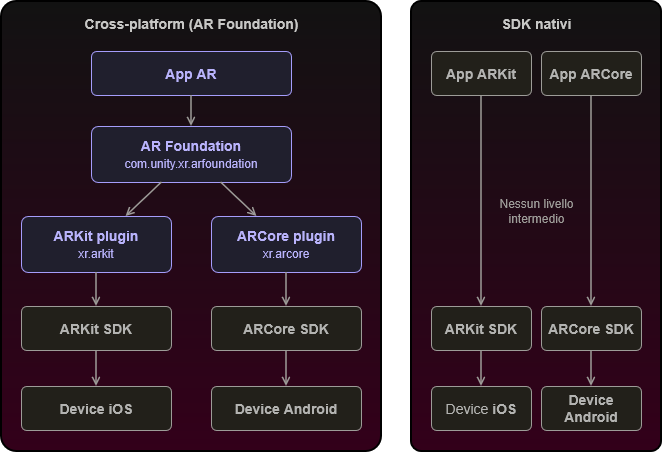
\includegraphics[width=0.7\textwidth]{images/ar-foundation/AR-Architecture.png}
    \caption{AR Foundation Architecture vs Native Architecture \cite{img-ar-foundation-architecture}}
    \label{fig:ar-architecture}
\end{figure}

\begin{itemize}
    \item \textbf{ARKit XR Plugin (\texttt{com.unity.xr.arkit})} e \textbf{ARCore XR Plugin (\texttt{com.unity.xr.arcore})}: package Unity ufficiali, gestiti tramite lo Unity Package Manager (UPM). Agiscono da \textit{provider} nell'architettura XR di Unity: contengono codice C\# e librerie native (\texttt{.a} per iOS, \texttt{.so} per Android) che fanno da ponte tra l'interfaccia astratta di AR Foundation e l'SDK nativo.

    \item \textbf{ARKit e ARCore (SDK nativi)}: non sono package Unity, ma i framework forniti da Apple e Google. Eseguono il tracciamento e la visione artificiale a basso livello: ARKit è integrato nel sistema operativo, mentre ARCore si appoggia al servizio di sistema Google Play Services for AR.

    \item \textbf{Accesso diretto alle funzioni native}: AR Foundation non funziona da sola, ma sempre tramite i provider. Per funzioni esclusive non ancora astratte, lo sviluppatore può usare le API esposte dai plug-in (ad esempio \texttt{ARKitSessionSubsystem} o \texttt{ARCoreSessionSubsystem}) senza scrivere plug-in C/C++ personalizzati. Per ARCore, funzioni come Geospatial e Cloud Anchors richiedono il package aggiuntivo \textbf{ARCore Extensions}.
\end{itemize}

Il vantaggio principale di AR Foundation è lo sviluppo con un'unica base di codice (\textit{single codebase}) valida sia per iOS sia per Android, che riduce tempi di sviluppo, manutenzione e costi di produzione. A ciò si aggiungono la rapidità di prototipazione, grazie alla configurazione dei componenti direttamente nell'editor di Unity, e l'integrazione nativa con l'ecosistema Unity: pipeline di rendering, profiler, sistema UI e Visual Scripting.

Gli svantaggi sono due. Il primo è che le novità hardware e le nuove API di Google o Apple non sono disponibili subito: bisogna attendere che Unity le supporti, e un ritardo in un aggiornamento o in un bugfix può bloccare il progetto. Il secondo è che il livello di astrazione introduce un overhead, con un impatto (generalmente contenuto) su framerate e uso di CPU e RAM.

L'approccio nativo con ARCore, privo di livelli intermedi, offre invece le massime prestazioni, un consumo di risorse minore, accesso immediato alle ultime funzionalità e integrazione profonda con i servizi della piattaforma, oltre all'accesso di basso livello a sensori, fotocamera e memoria. Il prezzo è però elevato: una curva di apprendimento più ripida, codice più verboso (\textit{boilerplate}), competenze specifiche per ciascuna piattaforma e una doppia manutenzione. Un'app con ARCore nativo funziona solo su Android, e per coprire iOS bisogna riscrivere la logica con ARKit, mantenendo due basi di codice da aggiornare e testare nel tempo.
\chapter{App}
\begin{figure}[H]
    \centering
    
    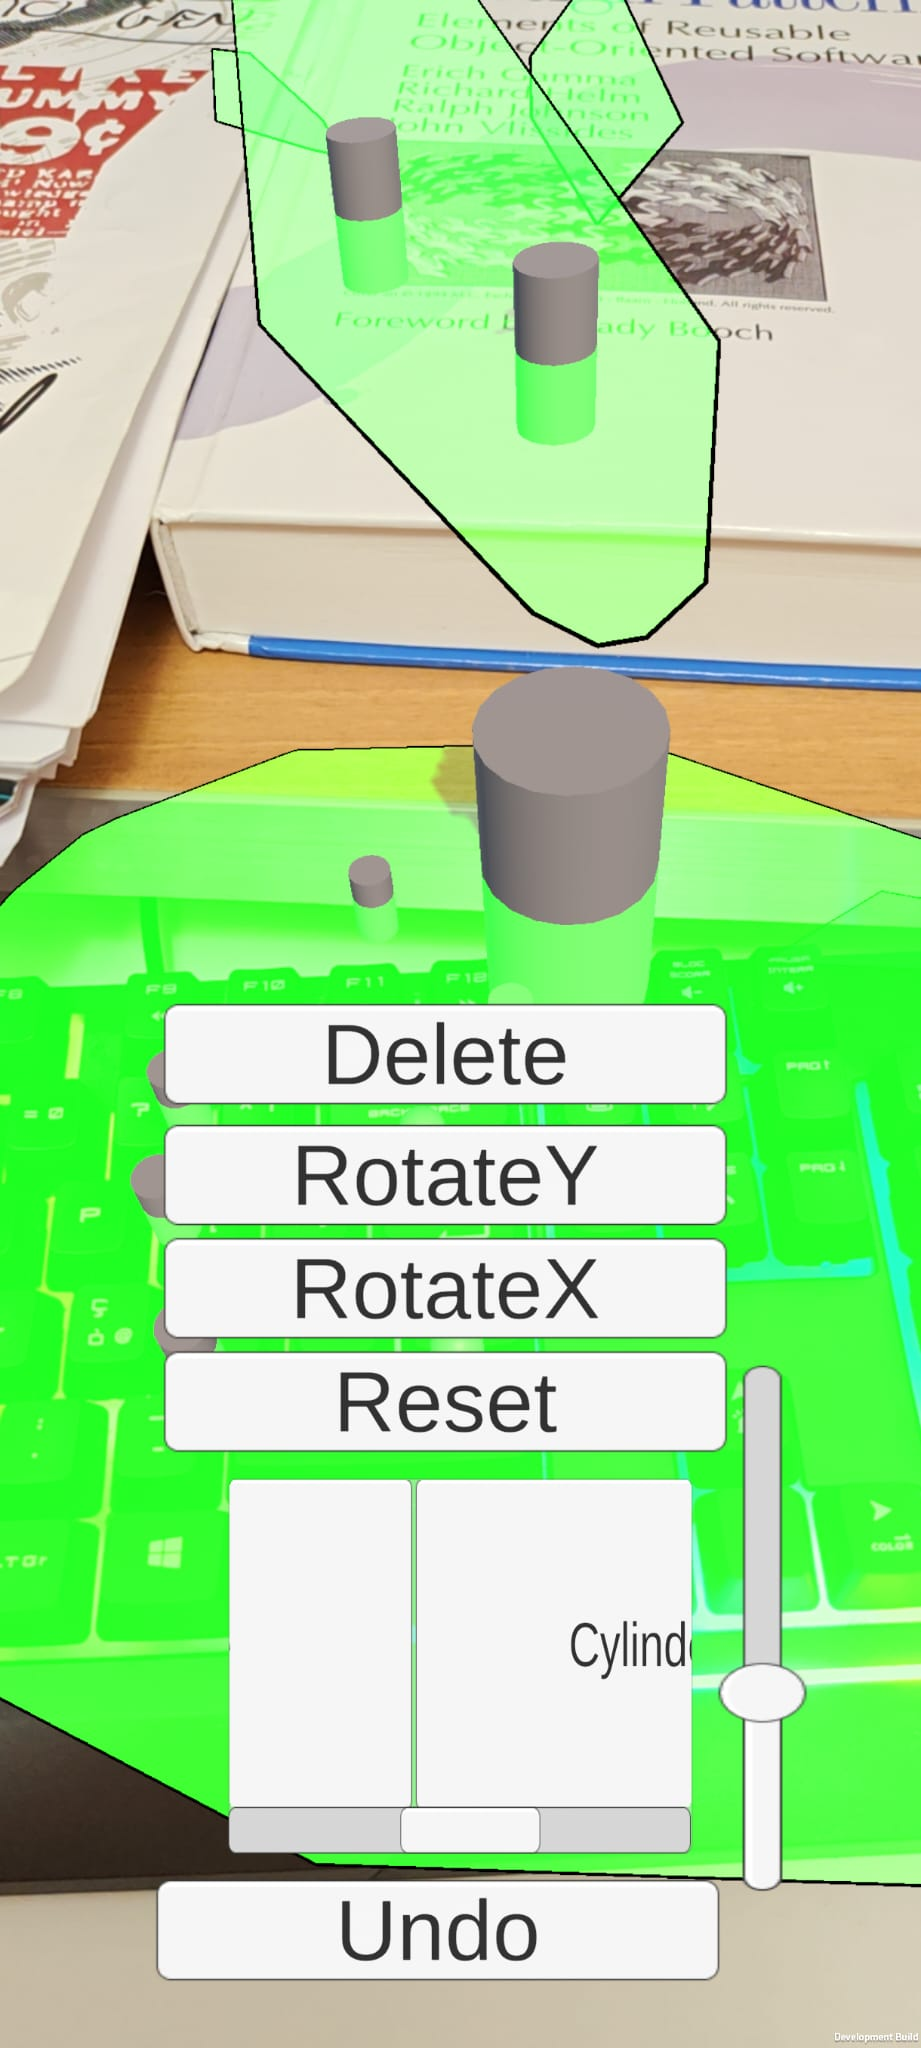
\includegraphics[width=0.4\textwidth]{images/app/MainAppInUseScreen.jpeg}
    \hfill 
    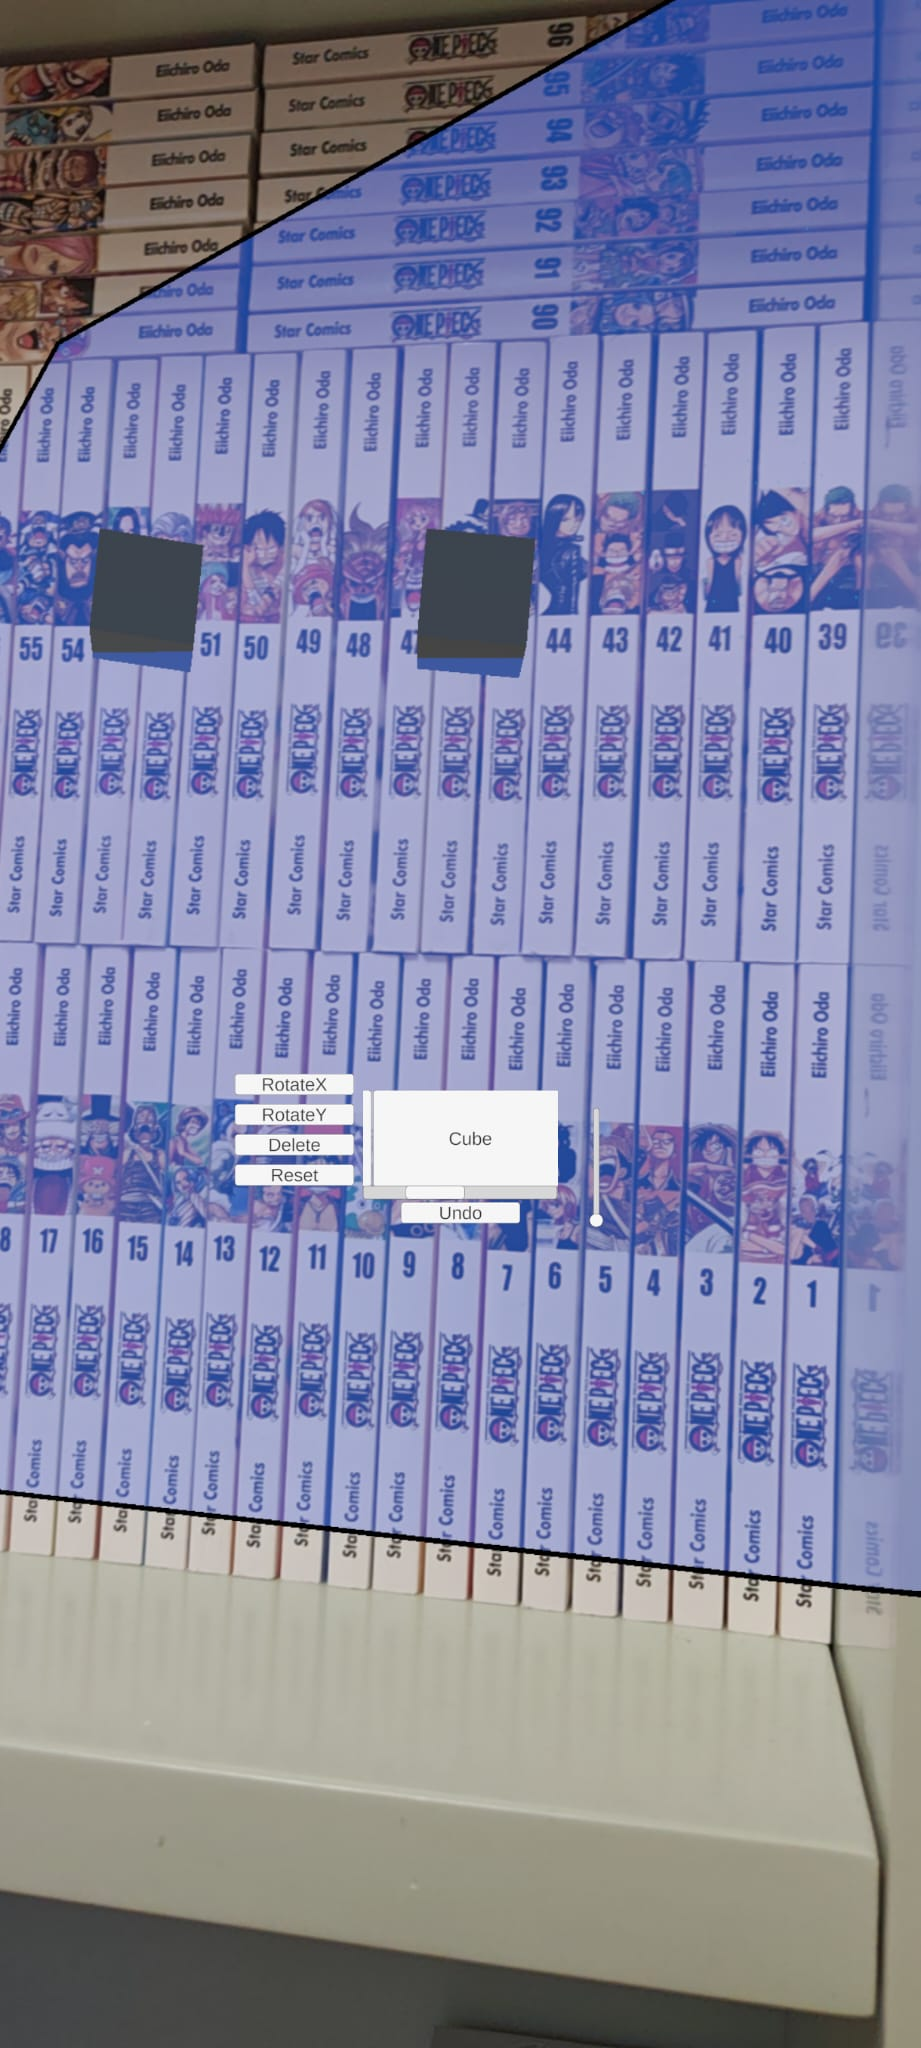
\includegraphics[width=0.4\textwidth]{images/app/ScreenInApp.jpeg} 
    
    
    \caption{Screenshots while my app is running on my phone}
    \label{fig:dt}
\end{figure}

    \begin{figure}[H]
        \centering
        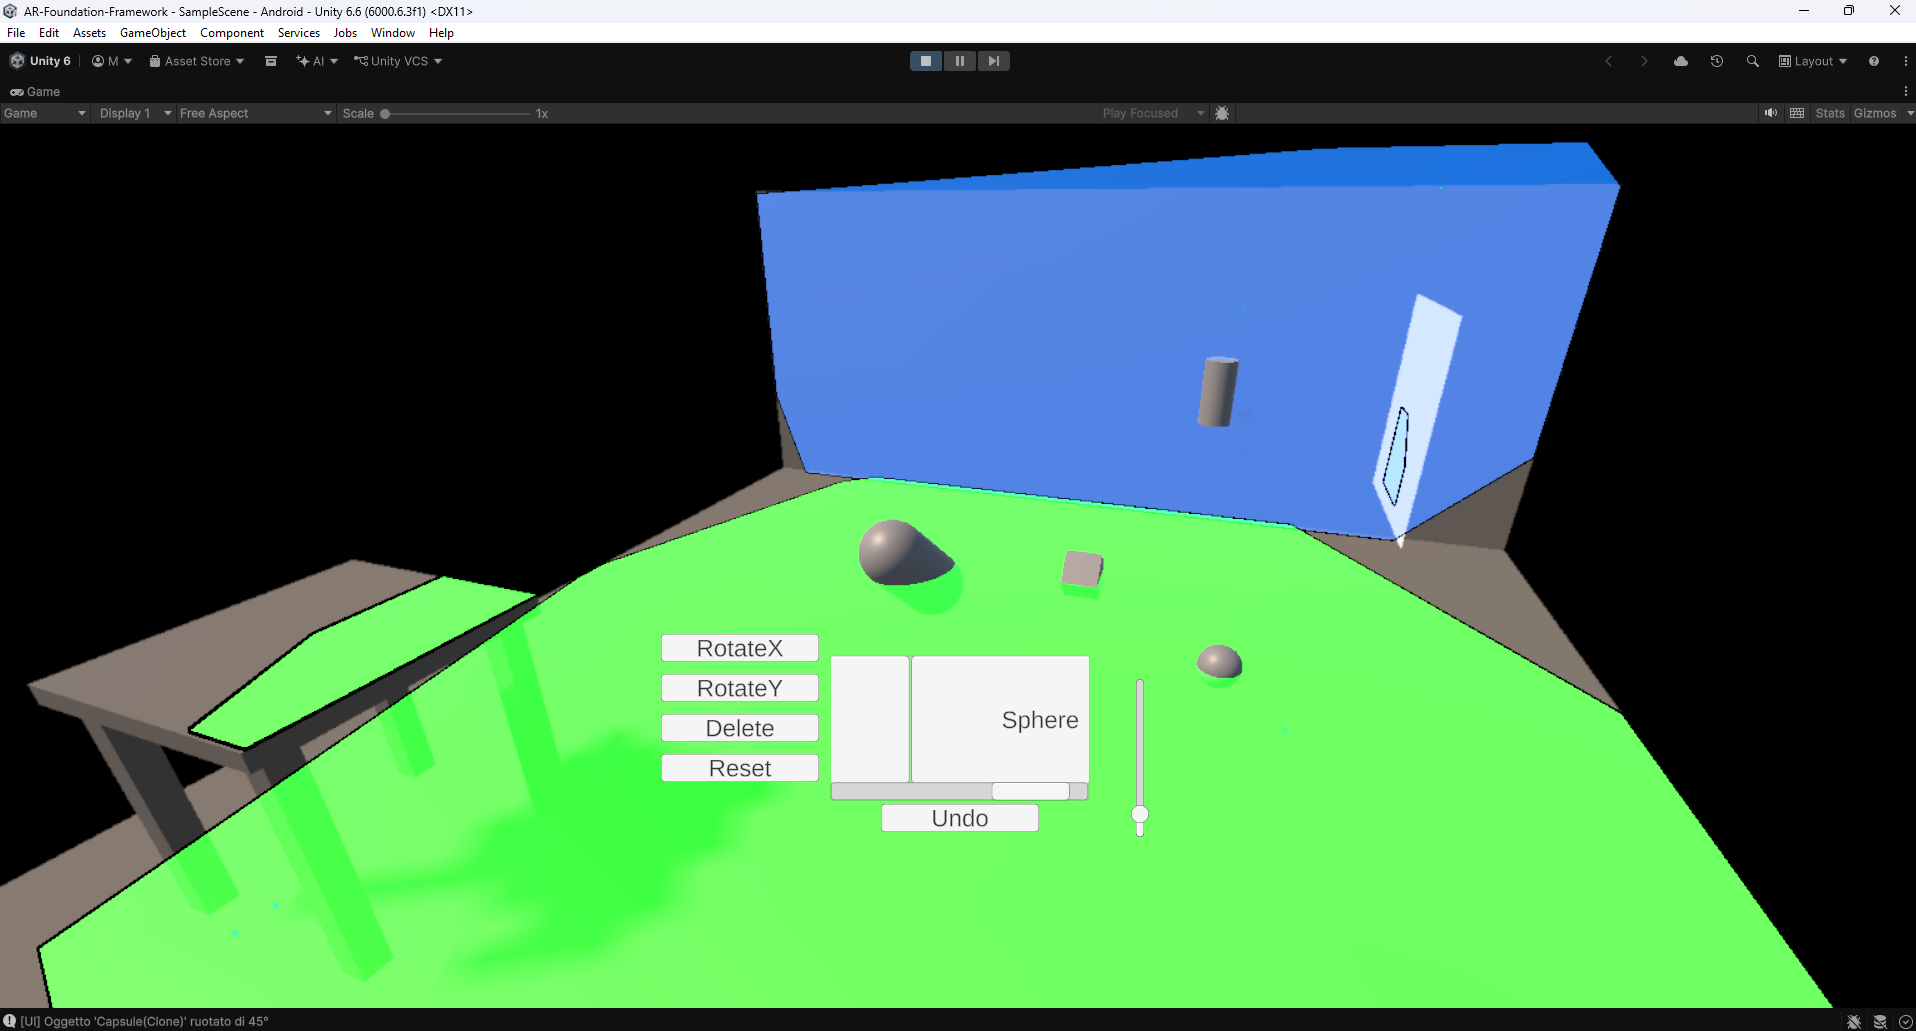
\includegraphics[width=0.7\textwidth]{images/app/AppInUseInEditor.png} 
        \caption{ Screen while my app is running in Unity XR Simulator}
        \label{fig:dt}
    \end{figure}


\section{Analisi Dei Requisiti}

\subsection{Scopo e Uso}
L'applicazione sviluppata in questo progetto è un app AR di tipo Markerless e Video See-Through, la quale consiste nella creazione dinamica di oggetti tridimensionali su superfici piane, con possibilità di eliminare, ruotare, scalare, spostare con drag and drop, pulire la scena e applicare \texttt{"l'undo"} alle azioni dell'utente (annullamento dell'azione), il quale interagisce tramite una semplice GUI composta da pulsanti, slider e per quanto riguarda \texttt{l'XR Simulator} con un input che prevede gestione del click del mouse, di una telecamera virtuale ARCamera e la possibilità di muoversi con WASD con la tastiera nell'editor di Unity e invece per quanto riguarda la distribuzione mobile del touch del touchscreen e della telecamera e sensori del cellulare.

Quest'app è stata distribuita su Android usando AR Foundation con ARCore XR Plug-In.
Come si può presumere, l'app distribuita su smartphone avrà un margine d'errore maggiore rispetto all'editor, derivato dal fatto che non si hanno superfici e telecamere/sensori ideali e stabili come nell'editor, infatti ciò può portare ad ulteriori ritardi, errori, saturazione e ha tanti altri fattori negativi. 

Per la realizzazione di tale software, ho fatto uso di 3 manager di AR principali, ovvero \texttt{ARPlane, ARRaycast e ARPointCloud} aggiunti come componenti all'\texttt{XR Origin}, con in aggiunta due manager custom creati da me per personalizzare \texttt{ARPlaneManager e ARPointCloudManager}, facendo in modo, rispettivamente, di vedere tre colori diversi per superfici verticali e orizzontali e quando l'oggetto è in stato di \texttt{"drag"} e stessa cosa per quanto riguarda i \texttt{"point cloud"}, un colore di default e l'altro quando il drag è attivo. Esempio di parte di codice usato per CustomPlaneManger: 
\begin{lstlisting}[language={[Sharp]C}]
public class CustomPlaneManager : MonoBehaviour
{
    //...
     private void OnPlanesChanged(ARTrackablesChangedEventArgs<ARPlane> args)
     {
         foreach (var plane in args.added)
             ApplyDefaultPlaneColor(plane);
         foreach (var plane in args.updated)
         {
             if (plane != currentlyActivePlane)
                 ApplyDefaultPlaneColor(plane);
         }
     }
    private void ApplyDefaultPlaneColor(ARPlane plane)
    {
        if (plane == null) return;
        Color targetColor = plane.alignment switch
        {
            PlaneAlignment.HorizontalUp or PlaneAlignment.HorizontalDown => horizontalColor,
            PlaneAlignment.Vertical => verticalColor,
            _ => defaultColor //_ scelta default
        };
        SetPlaneColor(plane, targetColor);
    }
    private void SetPlaneColor(ARPlane plane, Color color)
    {
        Renderer renderer = plane.GetComponent<Renderer>() ?? plane.GetComponentInChildren<Renderer>();
        if (renderer != null && renderer.material != null)
        {
            renderer.material.color = color;
        }
    }//...
}
\end{lstlisting}


In particolare, i 3 componenti AR usati sono: 
\begin{itemize}

    \item \textbf{ARPointCloudManager} serve a rilevare i "feature points" (punti di interesse), ovvero elementi visivi distintivi (angoli, trame, contrasti) che la fotocamera del dispositivo usa per orientarsi nello spazio; genera una "nuvola di punti" tridimensionale che rappresenta la struttura grezza dell'ambiente circostante e viene utilizzato principalmente dal sistema interno di tracciamento (SLAM) per capire come si muove il dispositivo ed è utile durante lo sviluppo o nelle fasi di calibrazione per mostrare all'utente che il sistema sta effettivamente "vedendo" l'ambiente.
    
    \item \textbf{ARPlaneManager} analizza la nuvola di punti e le immagini della fotocamera per identificare e ricostruire superfici piane reali; riconosce e traccia superfici piatte, classificandole automaticamente in piani orizzontali (es. pavimenti, tavoli), piani verticali (es. pareti, porte) e piani inclinati ed unisce automaticamente piani adiacenti se rileva che fanno parte della stessa superficie e aggiorna i loro confini in tempo reale man mano che l'utente inquadra l'ambiente. 

    \item \textbf{ARRaycastManager} permette di generare dei "raggi" virtuali dallo schermo del dispositivo verso l'ambiente reale per trovare punti di intersezione con gli elementi rilevati; esegue un test di collisione (raycasting) non contro i normali collider di Unity, ma contro i dati AR generati dall'ambiente (superfici tracciate dall'ARPlaneManager o feature points dell'ARPointCloudManager), per questo per il sistema di \texttt{drag and drop} degli oggetti ho fatto uso del raycast fisico che si basa sui collider; è essenziale per l'interazione dell'utente, poichè quando quest'ultimo tocca lo schermo, l'ARRaycastManager determina l'esatto punto nello spazio 3D reale in cui posizionare un oggetto.

\end{itemize}


\subsection{Requisiti Funzionali}

\subsubsection{RF1 - Interfaccia Grafica}
\begin{itemize}
    \item \textbf{RF1.1} - Il sistema deve mostrare i pulsanti che agiscono sull'oggetto, ovvero Delete, CleanAllObject, Rotate(x and y) and Spawn
    \item \textbf{RF1.2} - Il sistema deve mostrare il pulsante per l'annullamento delle azioni
    \item \textbf{RF1.3} - Il sistema deve mostrare una Scroll View per selezionare l'oggetto da spawnare
    \item \textbf{RF1.4} - Il sistema deve mostrare uno Slider per cambiare la scala di un oggetto selezionato a runtime
\end{itemize}

\subsubsection{RF2 - Sistema Di Input}
\begin{itemize}
    \item \textbf{RF2.1} - Il sistema deve avere accesso alla telecamera del dispositivo mobile oppure una camera virtuale di un simulatore
    \item \textbf{RF2.2} - Il sistema deve avere accesso a vari sensori del dispositivo
    \item \textbf{RF2.3} - Il sistema deve consentire all'utente di interagire tramite il touch da mobile (il movimento con WASD qua è camminare nel mondo reale) e con il mouse e tastiera(WASD) dal simulatore.
\end{itemize}

\subsubsection{RF3 - Sistema Di Output e Comportamento}
\begin{itemize}
    \item \textbf{RF3.1} - Il sistema deve poter intercettare e visualizzare a schermo le superfici piane(verticali, orizzontali o inclinati), in corrispondenza con il mondo reale
    \item \textbf{RF3.2} - Il sistema deve poter intercettare e visualizzare a schermo le varie point clouds, in corrispondenza con il mondo reale 
    \item \textbf{RF3.3} - Il sistema deve poter interpretare e capire quando vede un piano tramite operazione di Raycast
\end{itemize}

\subsection{Requisiti Non Funzionali}
\subsubsection{RNF1 – Usabilità}

\begin{itemize}
  \item \textbf{RNF1.1} - I comandi devono essere intuitivi e facilmente accessibili
    (\texttt{WASD}/frecce, mouse, pulsanti, scroll view, slider).
  \item RNF1.2 - L'interfaccia deve essere chiara e mostrare informazioni essenziali
    (comandi e output).
  \item RNF1.3 - Il sistema deve essere comprensibile senza necessità di un tutorial complesso.
\end{itemize}

\subsubsection{RNF2 – Affidabilità}  Il sistema non deve andare in crash durante una sessione di uso standard.


\subsubsection{RNF3 – Manutenibilità}
\begin{itemize}
  \item RNF3.1 - Il codice deve essere strutturato in moduli separati.
  \item RNF3.2 - Il sistema deve permettere l'aggiunta di nuovi prefab o nuove funzioni senza
    modificare pesantemente il codice esistente.
\end{itemize}

\subsubsection{RNF4 – Portabilità}

\begin{itemize}
  \item RNF4.1 - Il sistema deve essere eseguibile sui sistemi operativi scelti.
  \item RNF4.2 - Il sistema non deve dipendere da librerie non portabili o non supportate.
\end{itemize}

\subsubsection{RNF5 – Sicurezza}  Il sistema deve impedire input non validi o fuori dai limiti


\subsubsection{RNF6 – Qualità grafica} Gli asset grafici devono essere leggibili e non confondere l'utente.


\subsubsection{RNF7 – Scalabilità} Il sistema deve poter gestire l'aggiunta di ulteriori elementi senza degradare significativamente le prestazioni.

\subsection{UML Diagrams}
Ho diviso in più parti i diagrammi Activity e Class per renderli più visibili.
\begin{figure}[H]
        \centering
        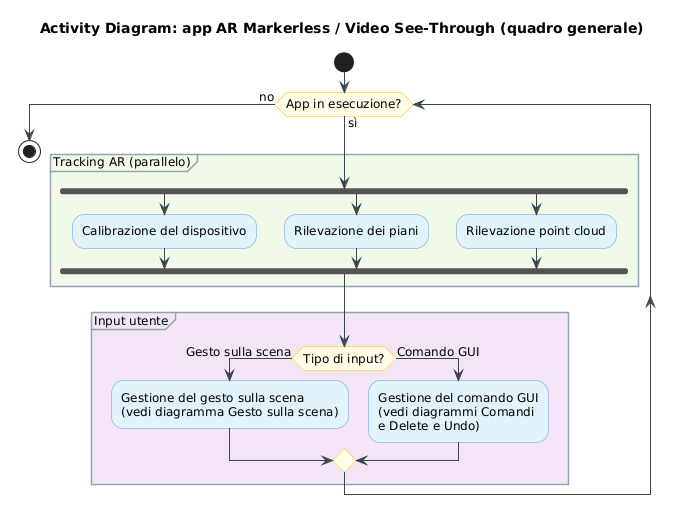
\includegraphics[width=0.7\textwidth, keepaspectratio]{images/app/ActivityDiagram_Generale.png} 
        \caption{ Activity Diagram, Focus: Generale}
        \label{fig:dt}
    \end{figure}

    \begin{figure}[H]
        \centering
        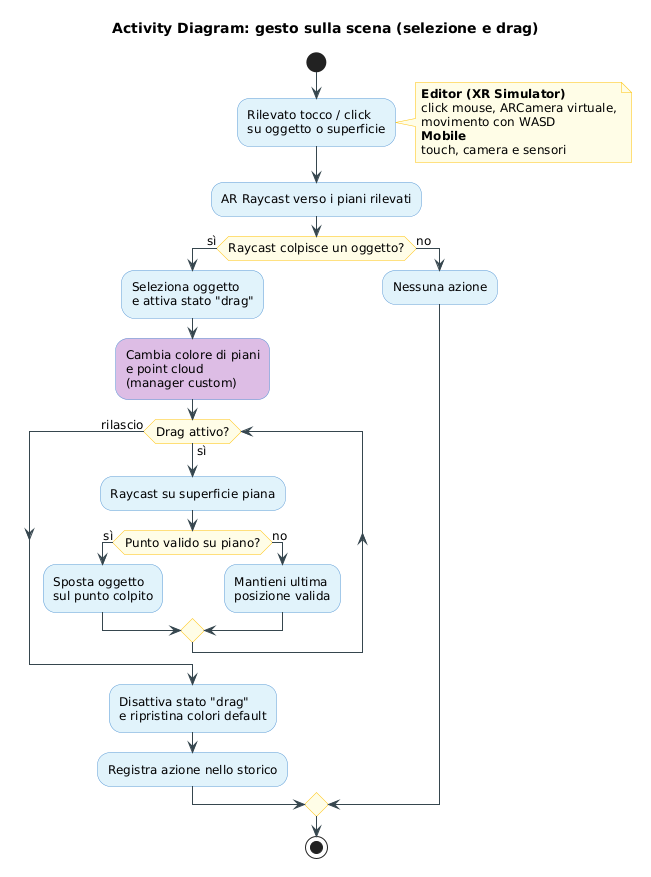
\includegraphics[width=0.7\textwidth, keepaspectratio]{images/app/ActivityDiagram_selezione_drag.png} 
        \caption{ Activity Diagram, Focus: Selezione e Drag}
        \label{fig:dt}
    \end{figure}
    
    \begin{figure}[H]
        \centering
        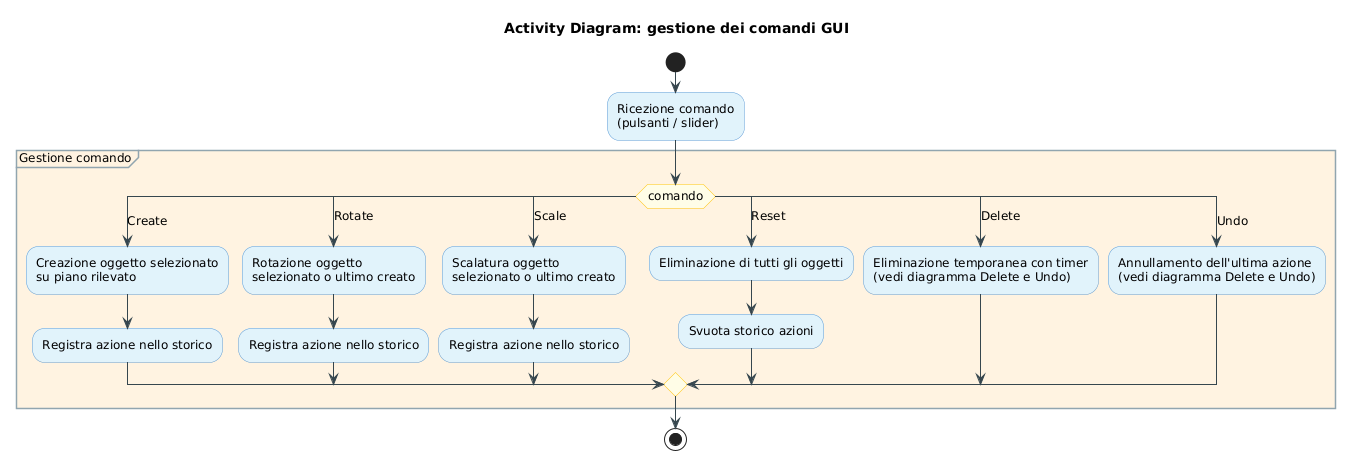
\includegraphics[width=0.7\textwidth, keepaspectratio]{images/app/ActivityDiagram_GUI.png} 
        \caption{ Activity Diagram, Focus: GUI}
        \label{fig:dt}
    \end{figure}

    \begin{figure}[H]
        \centering
        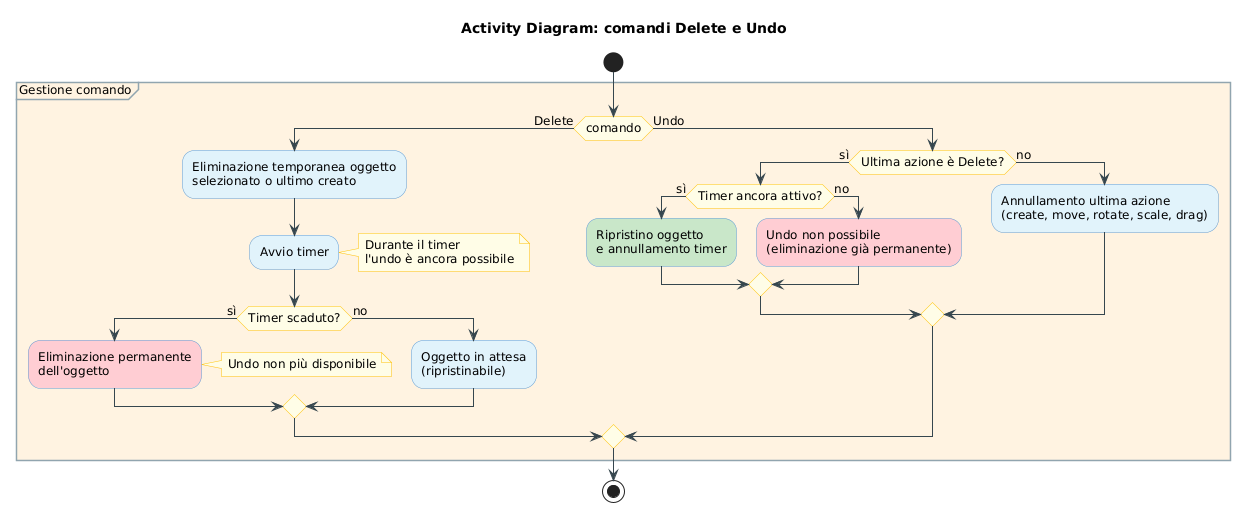
\includegraphics[width=0.7\textwidth, keepaspectratio]{images/app/ActivityDiagram_del_undo.png} 
        \caption{ Activity Diagram, Focus: GUI Delete e Undo}
        \label{fig:dt}
    \end{figure}

\begin{figure}[H]
        \centering
        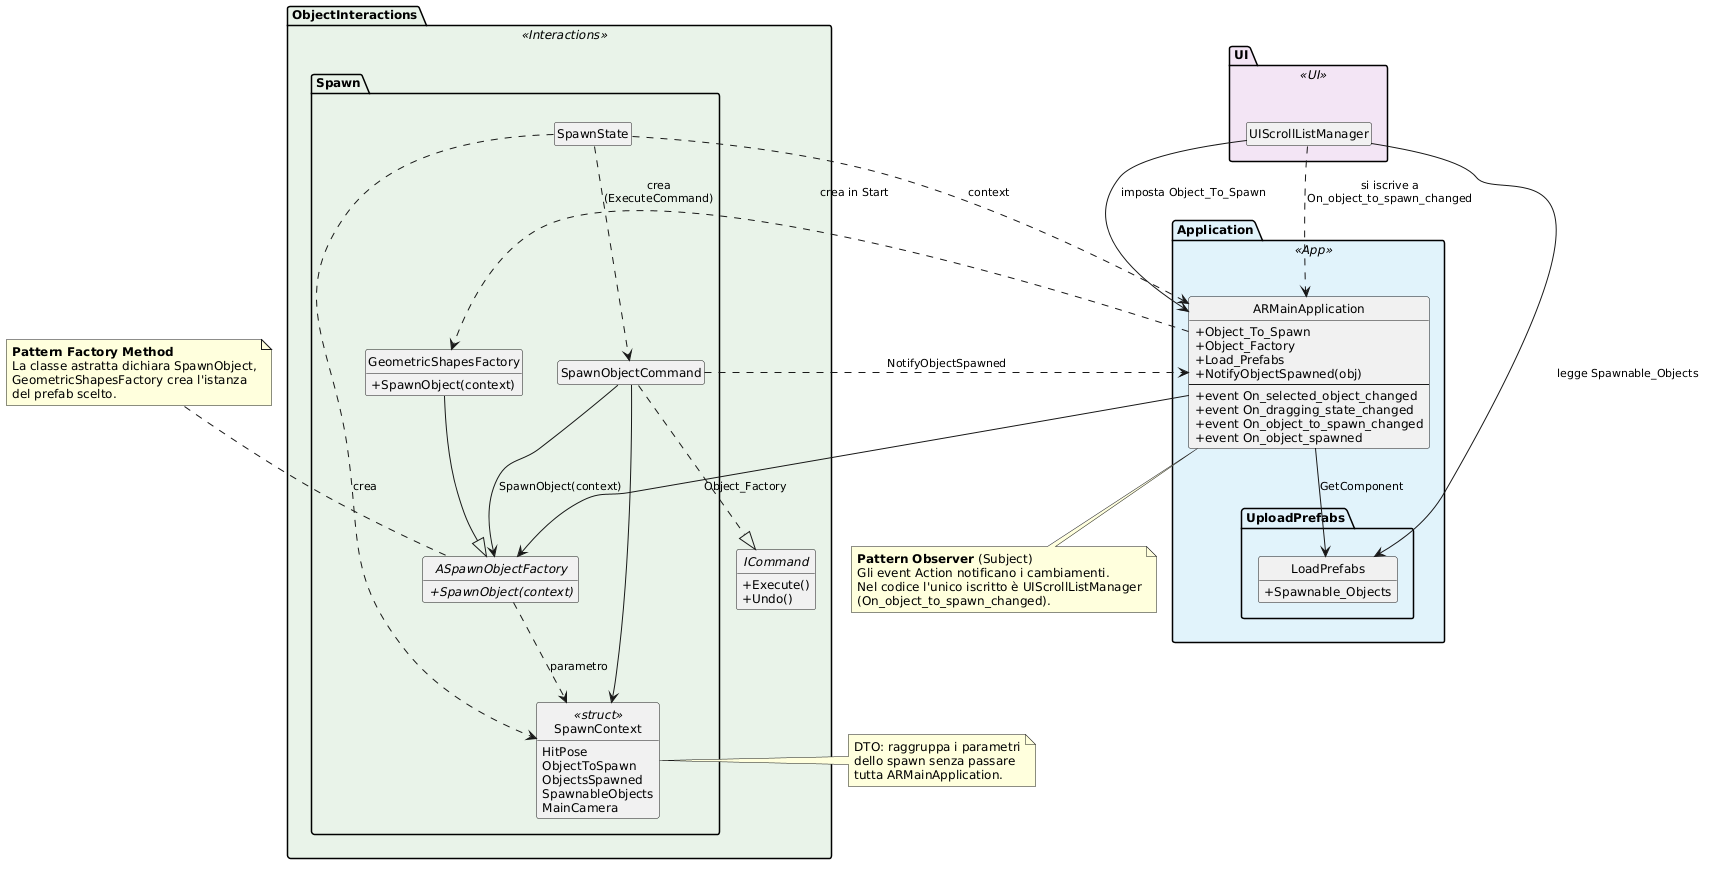
\includegraphics[width=1\textwidth, keepaspectratio]{images/app/ClassDiagram_Factory-Observer.png} 
        \caption{ Class Diagram, Focus: Factory e Observer}
        \label{fig:dt}
    \end{figure}

    \begin{figure}[H]
        \centering
        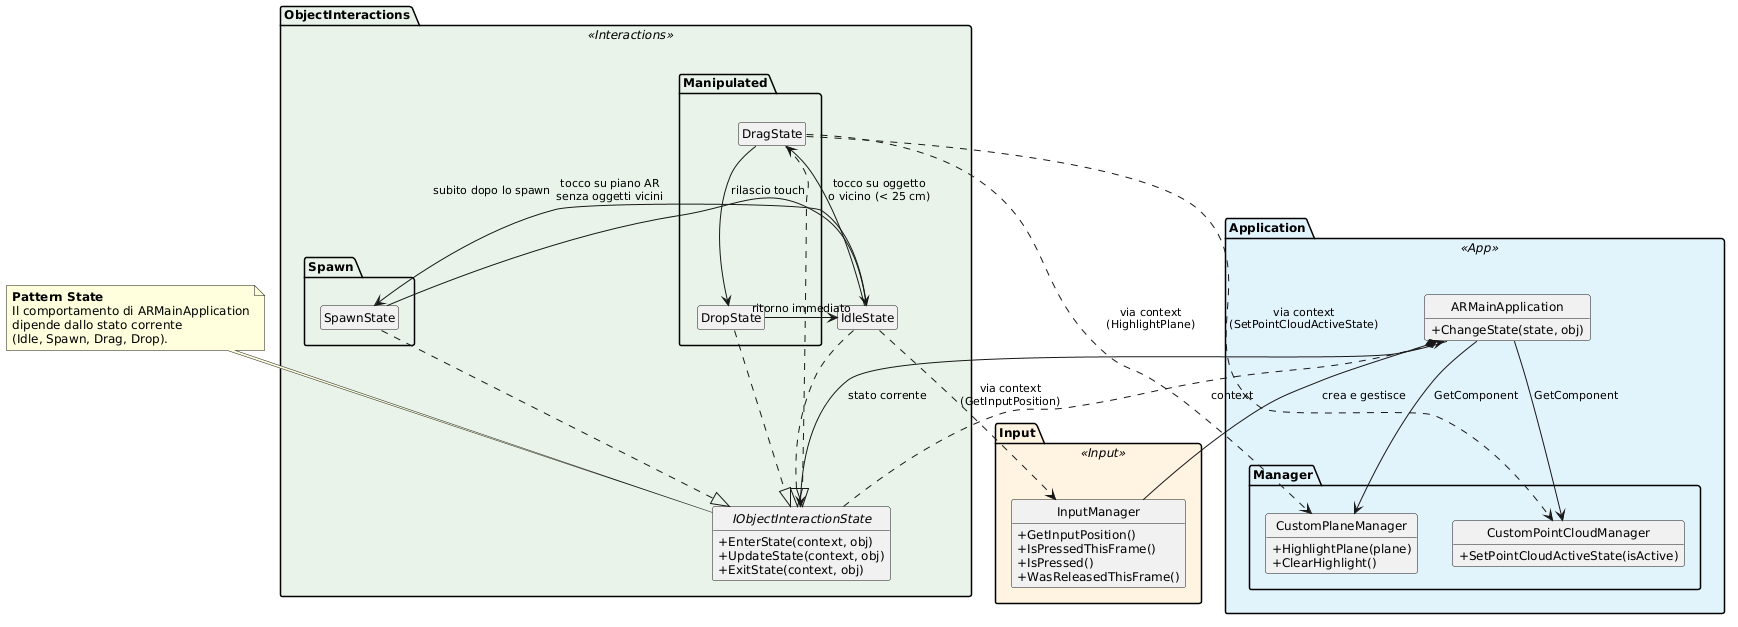
\includegraphics[width=1\textwidth, keepaspectratio]{images/app/ClassDiagram_State.png} 
        \caption{ Class Diagram, Focus: State}
        \label{fig:dt}
    \end{figure}

    \begin{figure}[H]
        \centering
        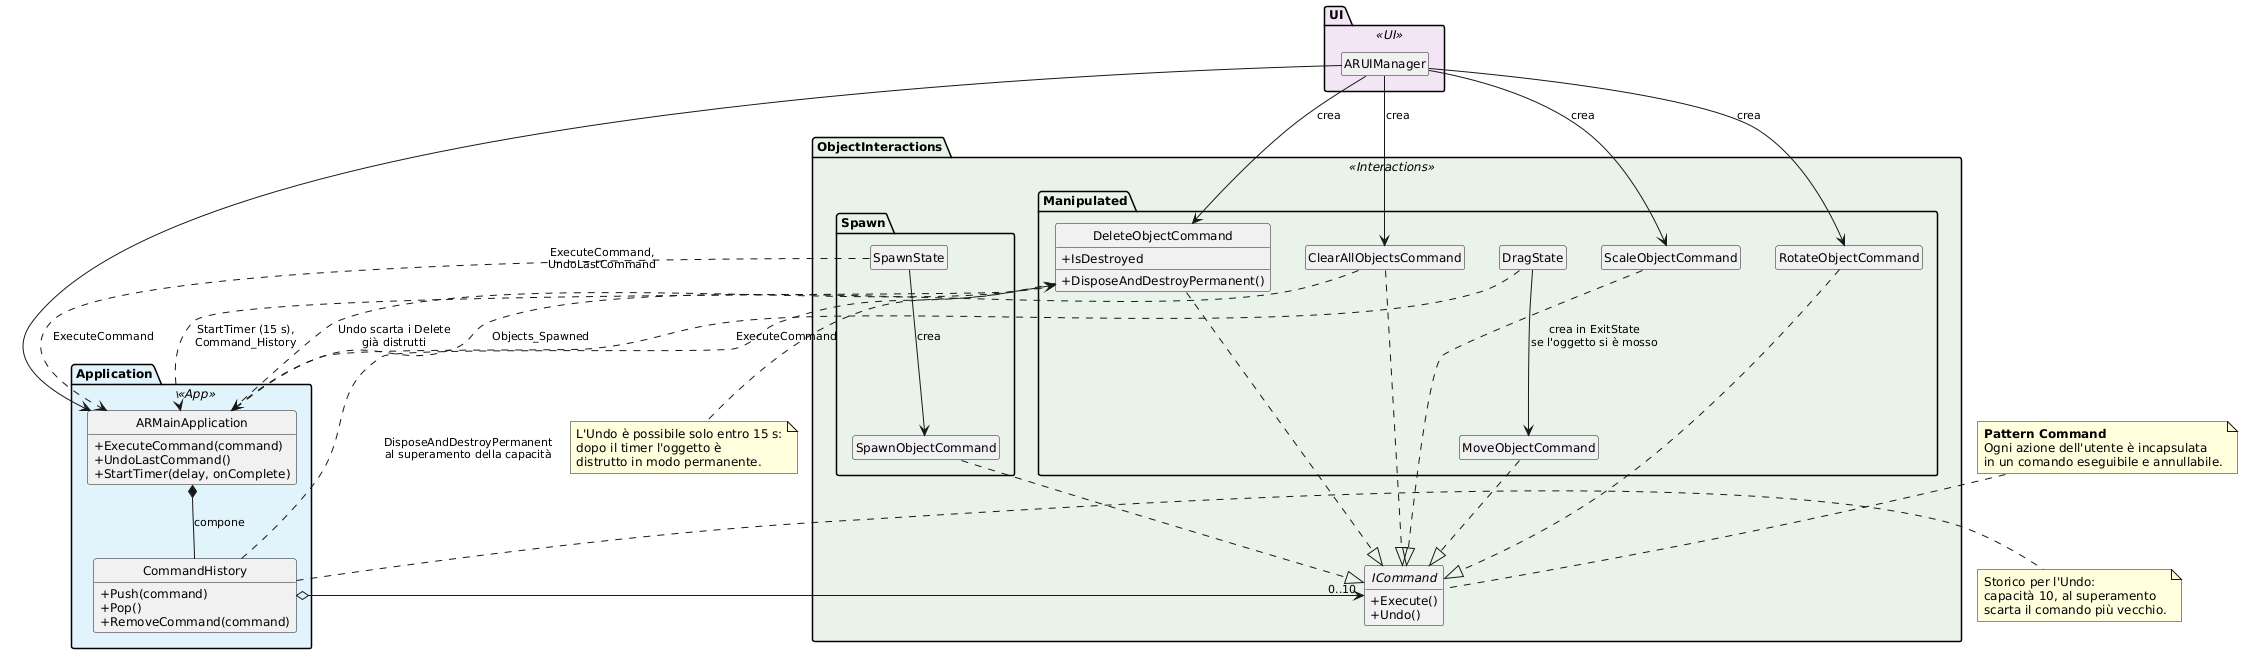
\includegraphics[width=1\textwidth, keepaspectratio]{images/app/ClassDiagram_Command.png} 
        \caption{ Class Diagram, Focus: Command}
        \label{fig:dt}
    \end{figure}
    
\section{Design Pattern}
\subsection{Convenzioni di Nomenclatura}

\begin{itemize}
  \item Le \textbf{classi astratte} sono prefissate con \texttt{A}.
  \item Le \textbf{interfacce} sono prefissate con \texttt{I}.
  \item I \textbf{metodi} e le \textbf{classi concrete} seguono \textit{QuestoCase}.
  \item Le \textbf{variabili} sono tutte minuscole con separatore \texttt{\_}.
  \item Le \textbf{variabili con Setter e Getter} sono tutte con l'iniziale maiuscola con separatore \texttt{\_}.
  \item le variabili evento observer Action (\textbf{eventi observer Action}) dell'engine sono con una sola iniziale maiuscola (obbligatorio) e il resto in minuscolo con separatore \texttt{\_}.
\end{itemize}

\subsection{Command}
Design pattern comportamentale e consente di incapsulare un'azione dentro ad un oggetto, diasaccopiando chi invoca l'azione da chi la esegue.
Nel progetto è stato usato per le azioni che può compiere l'utente, integrando anche il meccanismo di annullamento dell'azione (undo).
(Vedi in Factory Method per l'implementazione di un comando)
\begin{lstlisting}[language={[Sharp]C}]
public interface ICommand
{
    void Execute();
    void Undo();
}
\end{lstlisting}

\subsection{State}
Design pattern comportamentale e consente ad un oggetto di cambiare il proprio comportamento a runtime in base allo stato in cui si trova e quindi di cambiare anche quest'ultimo. Nel progetto è stato usato per rappresentare i vari stati diversi dell'interazione con gli oggetti.

\begin{lstlisting}[language={[Sharp]C}]
public interface IObjectInteractionState
{
    void EnterState(ARMainApplication context, GameObject obj);
    void UpdateState(ARMainApplication context, GameObject obj);
    void ExitState(ARMainApplication context, GameObject obj);
}

public class SpawnState : IObjectInteractionState
{
    public void EnterState(ARMainApplication context, GameObject obj)
    {
        if (context.Object_Factory != null && context.Hit_List.Count > 0)
        {
            Pose hit_pose = context.Hit_List[0].pose;
            SpawnContext spawn_context = new SpawnContext(
                hit_pose,
                context.Object_To_Spawn,
                context.Objects_Spawned,
                context.Load_Prefabs.Spawnable_Objects,
                context.Main_Camera
            );

            // Invece di chiamare direttamente lo Spawn, incapsuliamo nel Command
            ICommand spawn_cmd = new SpawnObjectCommand(context.Object_Factory, spawn_context, context);
            context.ExecuteCommand(spawn_cmd);
        }
        context.ChangeState(new IdleState(), null);
    }//...
}
public class ARMainApplication : MonoBehaviour
{
    //...
    public void ChangeState(IObjectInteractionState newState, GameObject targetObj)
    {
        current_state?.ExitState(this, targetObj);
        current_state = newState;
        current_state?.EnterState(this, targetObj);
    }
    //...
}
\end{lstlisting}

\subsection{Observer}
Design pattern comportamentale che definisce come gli oggetti comunicano quando uno cambia stato, notificando automaticamente tutti gli osservatori (Per Invoke guarda Factory Method).
Nel progetto è stato usato per condividere informazioni sugli stati dell’applicazione, come la modalità di trascinamento (dragging) o lo spawn di un nuovo oggetto, senza che le classi coinvolte si conoscano direttamente.

L’implementazione sfrutta i delegate di C\#: ARMainApplication espone eventi di tipo Action (ad esempio On\_dragging\_state\_changed), a cui gli altri componenti si iscrivono con l’operatore +=. La parola chiave event impedisce agli iscritti di invocare l’evento o di sovrascrivere gli altri osservatori, mantenendo l’incapsulamento. Quando lo stato cambia, il setter della proprietà richiama Invoke tramite l’operatore ?., che evita errori se nessun osservatore è iscritto. La notifica avviene solo se il valore è effettivamente cambiato, evitando chiamate inutili. In questo modo ARMainApplication (il subject) rimane disaccoppiato dagli osservatori, che possono essere aggiunti o rimossi senza modificarlo.

\begin{lstlisting}[language={[Sharp]C}]
public class ARMainApplication : MonoBehaviour
{
    public event Action<bool> On_dragging_state_changed;
    //...
     public bool Is_Dragging
     {
         get => is_dragging;
         set
         {
             if (is_dragging != value)
             {
                 is_dragging = value;
                 On_dragging_state_changed?.Invoke(is_dragging); // Notifica Observer
             }
         }
     }
     //...
    public void NotifyObjectSpawned(GameObject spawnedObj)
   {
       On_object_spawned?.Invoke(spawnedObj);
   }

}

\end{lstlisting}

\subsection{Factory Method}
Design Pattern creazionale che consente di creare oggetti senza specificare esplicitamente la loro classe concreta, delegando la creazione alle sottoclassi. Nel progetto è stato usato per la creazione di oggetti.
\begin{lstlisting}[language={[Sharp]C}]
public abstract class ASpawnObjectFactory
{
    public abstract GameObject SpawnObject(SpawnContext context);
}

public class SpawnObjectCommand : ICommand
{//...
    public void Execute()
    {
        spawned_object = factory.SpawnObject(spawn_context);
        if (spawned_object != null && ar_app != null)
        {
            ar_app.NotifyObjectSpawned(spawned_object);
        }
    }

    public void Undo()
    {
        if (spawned_object != null)
        {
            if (ar_app != null && ar_app.Objects_Spawned.Contains(spawned_object))
            {
                ar_app.Objects_Spawned.Remove(spawned_object);
            }
            Object.Destroy(spawned_object);
        }
    }
}
\end{lstlisting}



\subsection{Struttura Dati: CommandHistory}
è una struttura dati, creata da me, formata da una \texttt{LinkedList} di \texttt{ICommand}, implementato come uno stack, in modo da creare il meccanismo di \texttt{undo} ed eliminare l'undo o dei comandi per oggetti selezionabili che possono non coincidere con gli ultimi inseriti. 
\begin{lstlisting}[language={[Sharp]C}]
public class CommandHistory
{//...
    public void Push(ICommand command)
    {
        history.AddLast(command);
        // Se superiamo la capacita' massima, rimuoviamo il primo elemento (il piu' vecchio)
        if (history.Count > maxCapacity)
        {
            ICommand oldestCommand = history.First.Value;
            history.RemoveFirst();

            // Se il comando eliminato e' una cancellazione definitiva, puliamo la risorsa
            if (oldestCommand is DeleteObjectCommand deleteCmd)
            {
                deleteCmd.DisposeAndDestroyPermanent();
            }
        }
    }

    public ICommand Pop()
    {
        if (history.Count == 0) return null;

        ICommand lastCommand = history.Last.Value;
        history.RemoveLast();
        return lastCommand;
    }//...

    //Serve in DeleteObjectCommand, poiche' l'oggetto selezionato puo' essere diverso dall'ultimo messo
    public bool RemoveCommand(ICommand command)
    {
        if (command == null) return false;

        LinkedListNode<ICommand> node = history.Find(command);
        if (node != null)
        {
            history.Remove(node);
            Debug.Log("[CommandHistory] Comando rimosso con successo dallo storico!");
            return true;
        }
        Debug.LogWarning("[CommandHistory] Impossibile trovare il comando da rimuovere nello storico.");
        return false;
    }
}
\end{lstlisting}

\section{Analisi delle Prestazioni e Profiling}

Per la valutazione sperimentale e l'ottimizzazione dell'applicazione è stato impiegato il \textit{Unity Profiler}\cite{profiler}, strumento di diagnostica integrato nell'engine che monitora in tempo reale e con frequenza al frame (un \textit{frame} è ciascuna immagine prodotta e mostrata a schermo) il carico computazionale sulla CPU, l'occupazione della memoria (RAM e \textit{Managed Heap}) e l'efficienza della pipeline di rendering. Il suo scopo è isolare i colli di bottiglia (\textit{bottlenecks}) e stabilire se i rallentamenti siano imputabili all'elaborazione logica, alle chiamate di disegno verso la GPU o alla gestione delle risorse di memoria.

\begin{figure}[H]
        \centering
        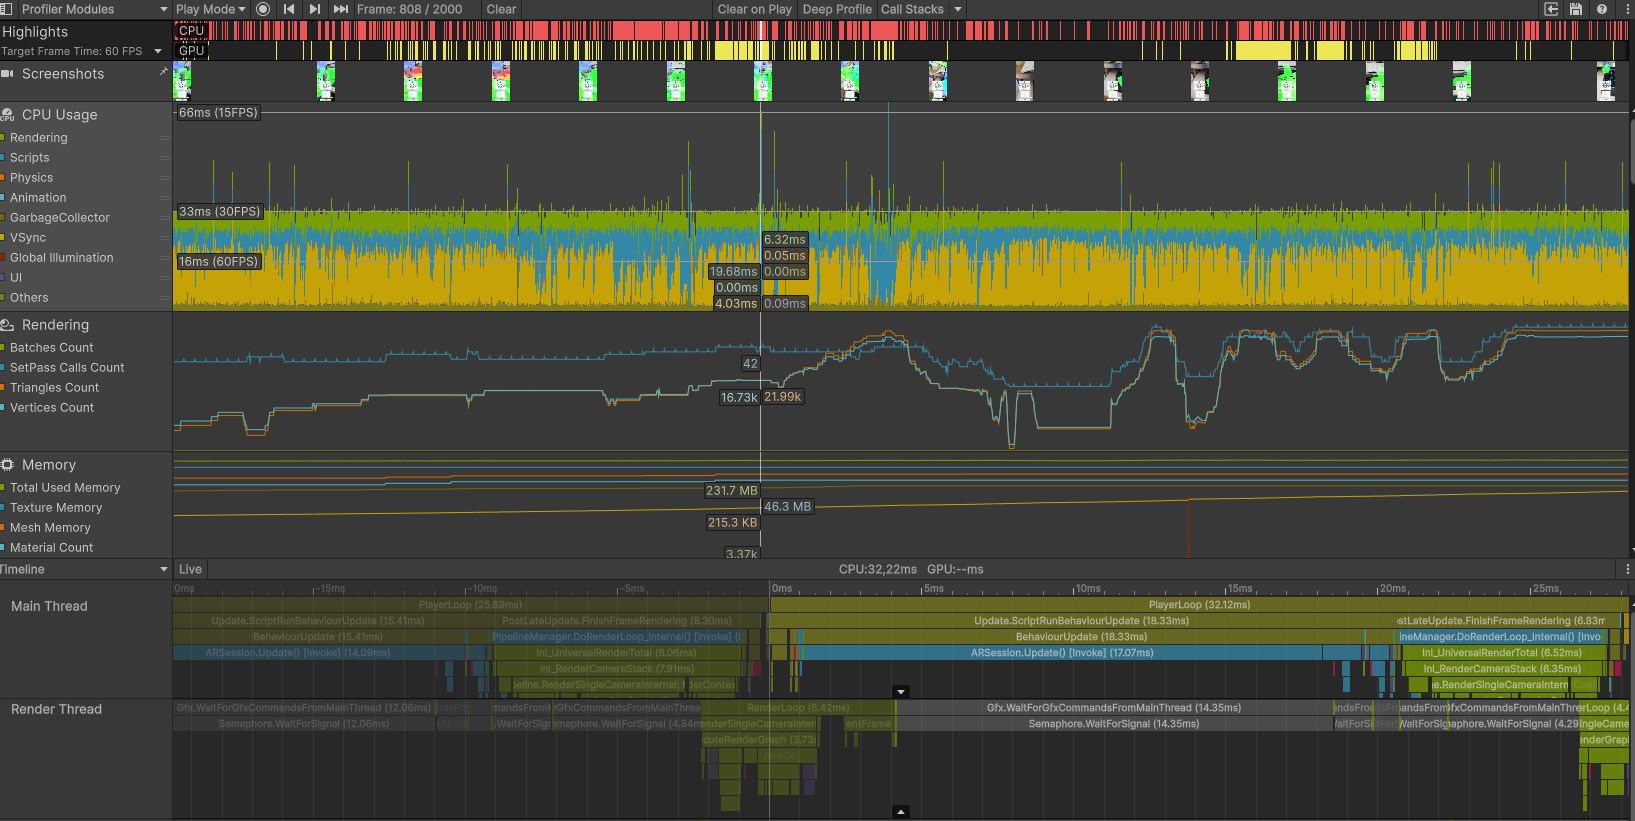
\includegraphics[width=0.7\textwidth]{images/app/GeneralStat.png} 
        \caption{Schermata generale dell'Unity Profiler durante l'esecuzione dell'applicazione sul dispositivo di test.}
        \label{fig:generalstat}
\end{figure}

I test sono stati condotti \textit{on-device} (direttamente sul dispositivo fisico e non nell'Editor di Unity), tramite build di debug collegata via ADB (\textit{Android Debug Bridge}, strumento di comunicazione tra computer e dispositivo Android) ad un dispositivo di fascia medio-alta, un \textbf{Motorola Edge 70} con:
\begin{itemize}
\item \textbf{Sistema Operativo:} Android 16.
\item \textbf{SoC e CPU:} Qualcomm Snapdragon 7 Gen 4 (\textit{SoC}, \textit{System on Chip}: unico chip che integra CPU, GPU ($1.15\text{ GHz}$) e altri componenti), Octa-Core, con clock fino a $2.8\text{ GHz}$.
\item \textbf{GPU:} Adreno 722.
\item \textbf{RAM:} $12\text{ GB}$ LPDDR5X (memoria RAM per dispositivi mobili, a basso consumo).
\item \textbf{Sensori coinvolti nel tracciamento:} fotocamera, accelerometro, giroscopio e magnetometro, con un Sensor Hub dedicato (coprocessore a basso consumo che raccoglie i dati dei sensori) per la fusione dei dati di tracciamento \textit{spatially-aware} (consapevole della posizione e dell'orientamento del dispositivo nello spazio).
\end{itemize}

\subsection{Tipologie di Grafici e Metodologia di Lettura}

Il profiler organizza la diagnostica in quattro tipologie di grafici, a diversi livelli di astrazione (dall'andamento temporale macroscopico al singolo microsecondo di esecuzione):

\begin{enumerate}
\item \textbf{Grafico ad Area Impilata (\textit{Timeline Stacked Area Chart}):} presente nel modulo \textit{CPU Usage}. Sull'asse $x$ sono riportati i frame sequenziali, sull'asse $y$ il tempo di esecuzione in $\text{ms}$. Le macro-categorie sono aree cromatiche sovrapposte: \textit{Scripts} (codice C\# eseguito, compreso quello dei package come AR Foundation, che nel frame analizzato ne costituisce la parte prevalente.), \textit{Rendering} (preparazione dei comandi grafici da parte della CPU), \textit{Garbage Collector} (meccanismo che libera automaticamente la memoria degli oggetti C\# non più usati, sospendendo temporaneamente il codice), \textit{Physics} (simulazione fisica), \textit{VSync} (attesa della sincronizzazione con l'aggiornamento del display) e \textit{UI} (interfaccia utente). Le linee orizzontali a $16\text{ ms}$ ($60\text{ FPS}$) e $33\text{ ms}$ ($30\text{ FPS}$) permettono di vedere il superamento della soglia del frame e l'impatto di ciascun sottosistema.

\item \textbf{Grafico a Linee (\textit{Line Chart}):} usato nei moduli \textit{Rendering} e \textit{Memory}, mostra l'andamento nel tempo di conteggi e quantità (ad esempio batch, triangoli, memoria usata) frame per frame.

\item \textbf{Traccia di Esecuzione e Threading (\textit{Flame Graph / Call Stack Timeline}):} nella sezione inferiore del profiler è una traccia a blocchi gerarchici annidati analoga a un diagramma di Gantt. Mostra due thread: il \textit{Main Thread} (thread principale, che esegue logica, script e preparazione dei comandi grafici) e il \textit{Render Thread} (thread dedicato che traduce tali comandi in chiamate alla GPU). L'asse orizzontale misura la cronologia interna del singolo frame (in $\text{ms}$), mentre le righe mostrano le chiamate a funzione e l'esecuzione parallela sui thread, evidenziando stalli e sincronizzazioni (\texttt{WaitForGfx\allowbreak Commands}, \texttt{Semaphore.\allowbreak WaitForSignal}).

\item \textbf{Grafici a Barre e Distribuzione Statistica (\textit{Breakdown Bar Charts e Highlights}):} usati in \textit{Selection Highlights}, \textit{Capture Highlights} e \textit{Memory Breakdown}. Barre orizzontali proporzionali mostrano valore assoluto e percentuale delle risorse, con indicatori statistici (minimo, mediana, massimo) per valutare la stabilità della sessione. La mediana è il valore centrale: metà dei frame è più veloce e metà più lenta.
\end{enumerate}

\subsection{Testing}
La cattura analizzata comprende $2000$ frame. Il frame time minimo è $19.198\text{ ms}$, quindi nessun frame rispetta il budget di $16.67\text{ ms}$ richiesto da un target di $60\text{ FPS}$, e la mediana è $33.408\text{ ms}$ (circa $30\text{ FPS}$). Il carico risulta più spesso limitato dalla CPU che dalla GPU (\textit{CPU-bound}, cioè una condizione in cui la velocità di generazione dei frame è limitata dal tempo impiegato dal processore per eseguire il codice e preparare i dati), ma, come mostrano i dati aggregati (\textit{Capture Highlights}), una parte rilevante del tempo di frame è attesa di sincronizzazione e non lavoro computazionale. Le analisi di dettaglio sono state svolte sul frame $808$, scelto perché il suo tempo di CPU ($32.782\text{ ms}$) è prossimo alla mediana della cattura ($33.408\text{ ms}$) e quindi rappresentativo della condizione tipica.

\subsubsection{Analisi del Frame Selezionato}

\paragraph{CPU Usage e profilo temporale.} Il modulo \textit{CPU Usage} misura il tempo necessario alla CPU per completare le operazioni di ciascun frame. A fronte di un target di $60\text{ FPS}$ (budget $\le 16.67\text{ ms}$), l'andamento supera costantemente tale soglia, posizionandosi spesso attorno ai $33\text{ ms}$ ($30\text{ FPS}$). Tale valore può essere influenzato anche da un limite alla frequenza di aggiornamento (\texttt{Application.\allowbreak targetFrameRate}, VSync o cadenza del flusso video di ARCore, la piattaforma Google per la realtà aumentata su Android su cui poggia AR Foundation) e non dipendere solo dal sovraccarico della CPU. La traccia del \textit{Main Thread} nel frame $808$ è così ripartita:

\begin{center}
\small
\begin{tabular}{|p{4.4cm}|p{6.8cm}|p{2.6cm}|}
\hline
\textbf{Routine} & \textbf{Funzione} & \textbf{Durata} \\
\hline
\texttt{Update.\allowbreak ScriptRun\allowbreak Behaviour\allowbreak Update} & Invoca il metodo \texttt{Update()} (eseguito una volta per frame) di tutti i \texttt{MonoBehaviour} attivi, cioè gli script Unity: punto d'ingresso del codice C\# e core della logica. Include le routine della riga seguente. & $18.33\text{ ms}$ \\
\hline
\texttt{ARSession.\allowbreak Update()}, \texttt{ARCameraManager.\allowbreak Update()} & Routine di AR Foundation (livello di Unity che unifica le piattaforme AR, qui basato su ARCore): sincronizzano e analizzano i dati di tracciamento (\textit{feature points}, cioè punti caratteristici dell'immagine usati per stimare la posa del dispositivo, piani rilevati) e convertono i frame video della fotocamera. & fino a $17.07\text{ ms}$ \\
\hline
\texttt{PostLate\allowbreak Update.\allowbreak Finish\allowbreak Frame\allowbreak Rendering} & Il \textit{Main Thread} impacchetta i comandi grafici e li inoltra alla coda del \textit{Render Thread}. & $6.83\text{ ms}$ \\
\hline
\texttt{Gfx.WaitForGfx\allowbreak Commands\allowbreak From\allowbreak MainThread}, \texttt{Semaphore.\allowbreak WaitFor\allowbreak Signal} (\textit{Render Thread}) & Il \textit{Render Thread} attende inattivo che il \textit{Main Thread} termini il frame; il semaforo è un meccanismo di sincronizzazione a basso livello tra thread. & $14.35\text{ ms}$ \\
\hline
\end{tabular}
\end{center}

Le durate sono \textit{inclusive} e annidate: \texttt{ARSession.Update()} viene eseguita all'interno di \texttt{BehaviourUpdate}, quindi i valori non vanno sommati. Ne deriva che la quasi totalità del tempo speso negli \texttt{Update()} ($17.07$ su $18.33\text{ ms}$) è dovuta ad AR Foundation e non agli script applicativi. Le attese del \textit{Render Thread} confermano che esso resta in attesa del completamento dei calcoli sul \textit{Main Thread}.

\paragraph{Rendering e complessità geometrica.} 

\begin{figure}[H]
        \centering
        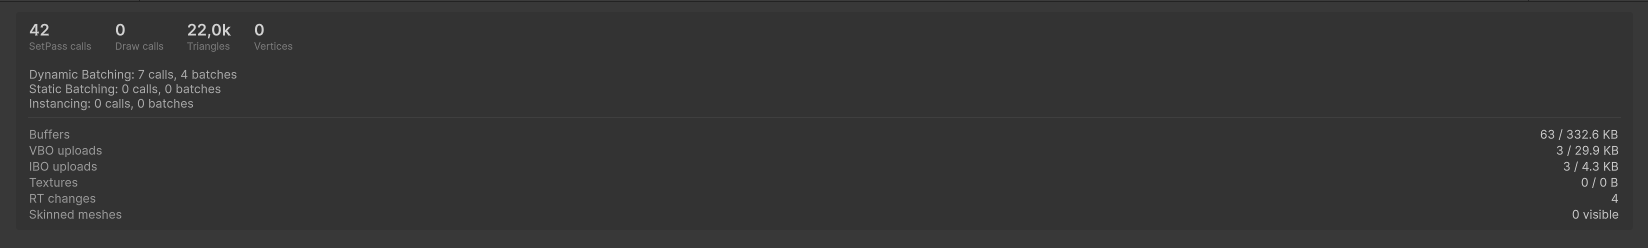
\includegraphics[width=0.8\textwidth]{images/app/RenderingStat.png} 
        \caption{Scheda \textit{Rendering} dell'Unity Profiler.}
        \label{fig:highlightsselection}
\end{figure}

Dai dati del modulo \textit{Rendering} il carico grafico risulta contenuto e non rappresenta il principale collo di bottiglia. Il \textit{Frame Debugger} (strumento che mostra frame per frame la sequenza dei comandi grafici inviati alla GPU) è raggiungibile dallo stesso modulo. I \textit{SetPass Calls}, cioè i cambi di stato di rendering (shader, texture, blending) che comportano un overhead per la CPU, sono $42$, valore molto contenuto per un dispositivo mobile. Il batching dinamico (tecnica che unisce oggetti semplici in un unico gruppo da disegnare, detto \textit{batch}) ha raggruppato $7$ chiamate di disegno in $4$ batch. La \textit{Universal Render Pipeline} (URP) adotta inoltre l'\textit{SRP Batcher}, meccanismo distinto dal batching dinamico che riduce il costo CPU dei cambi di materiale. La geometria conta $22.0\text{k}$ triangoli e $16.73\text{k}$ vertici, cifre che escludono problemi di saturazione della banda di memoria o di geometria eccessiva. Il \textit{GPU Time} non è disponibile per il frame selezionato (\textit{No Value}): la valutazione del carico grafico si basa quindi sulle statistiche di rendering e non su una misura diretta del tempo di GPU.

\paragraph{Memory e Managed Heap.} 
\begin{figure}[H]
        \centering
        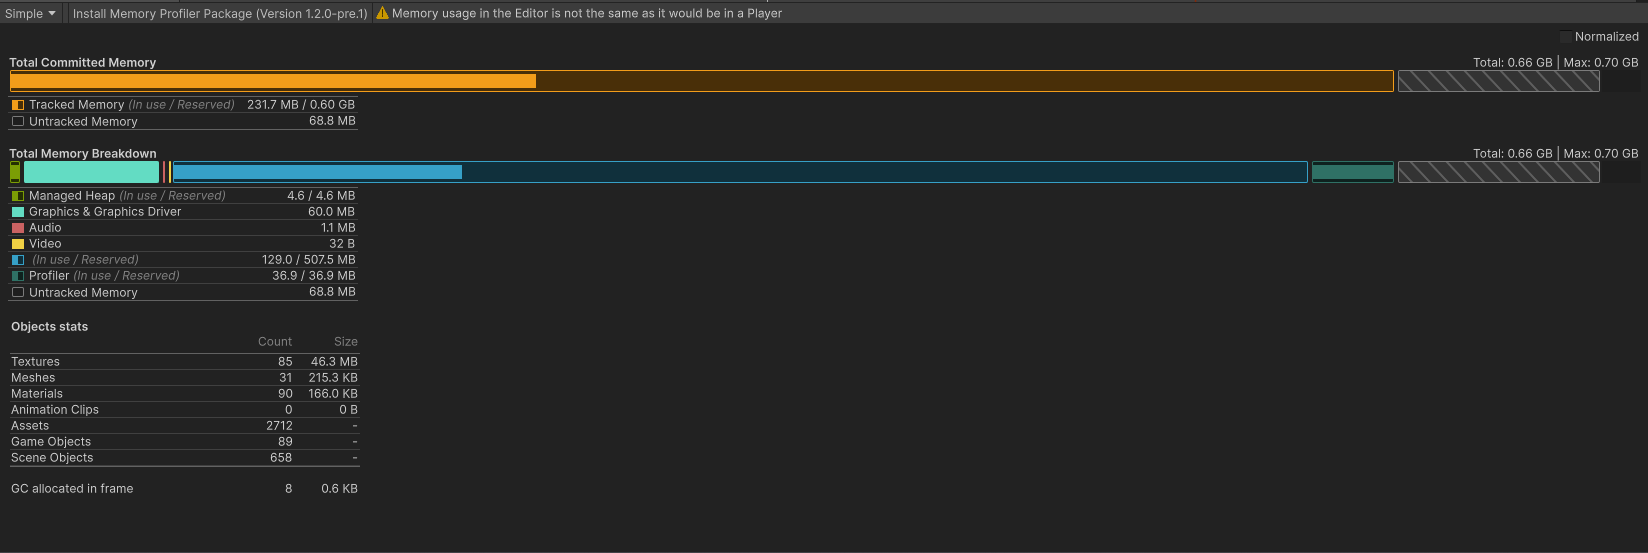
\includegraphics[width=0.8\textwidth]{images/app/MemoryStat.png} 
        \caption{Scheda \textit{Memory} dell'Unity Profiler.}
        \label{fig:highlightsselection}
\end{figure}

Il modulo distingue la memoria nativa di Unity (C++) dal \textit{Managed Heap}, l'area di memoria in cui vengono allocati gli oggetti C\# e la cui liberazione è affidata al \textit{Garbage Collector} (GC) invece che al programmatore. I consumi globali sono ben controllati, ma critici nelle allocazioni temporanee:
\begin{itemize}
\item \textbf{Total Committed Memory:} $0.66\text{ GB}$ su un massimo di $0.70\text{ GB}$. Indica la memoria complessivamente impegnata dall'applicazione, cioè richiesta al sistema operativo.
\item \textbf{Tracked Memory:} $231.7\text{ MB}$ in uso su $0.60\text{ GB}$ riservati. È la memoria che Unity sa attribuire a oggetti e sistemi; \textit{reserved} indica lo spazio già ottenuto dal sistema operativo, anche se non ancora in uso. A questa si aggiungono $68.8\text{ MB}$ di \textit{Untracked Memory}, non attribuibili da Unity (ad esempio plugin nativi e driver).
\item \textbf{Texture e Mesh:} $46.3\text{ MB}$ per $85$ texture (immagini applicate alle superfici); $215.3\text{ KB}$ per $31$ mesh (modelli geometrici 3D).
\item \textbf{Managed Heap e Garbage Collection:} $4.6\text{ MB}$ in uso, ma con allocazioni continue ad ogni frame: nel frame selezionato $9$ allocazioni per $0.7\text{ KB}$ (\textit{GC Alloc}), originate principalmente da \texttt{Draw AR Background} ($376\text{ B}$) e dal \textit{Render Graph} ($128\text{ B}$); sull'intera cattura le allocazioni sono $18.119$, con un massimo di $43.9\text{ KB}$ in un singolo frame (frame $1396$) e routine di AR Foundation tra i principali contributori. Il valore istantaneo è ridotto, ma l'accumulo genera frequenti interventi bloccanti del GC, che sospende l'esecuzione del codice C\# per ripulire la memoria non più utilizzata.
\end{itemize}

\subsubsection{Analisi Statistica degli Highlights (Selection e Capture)}
\begin{figure}[H]
        \centering
        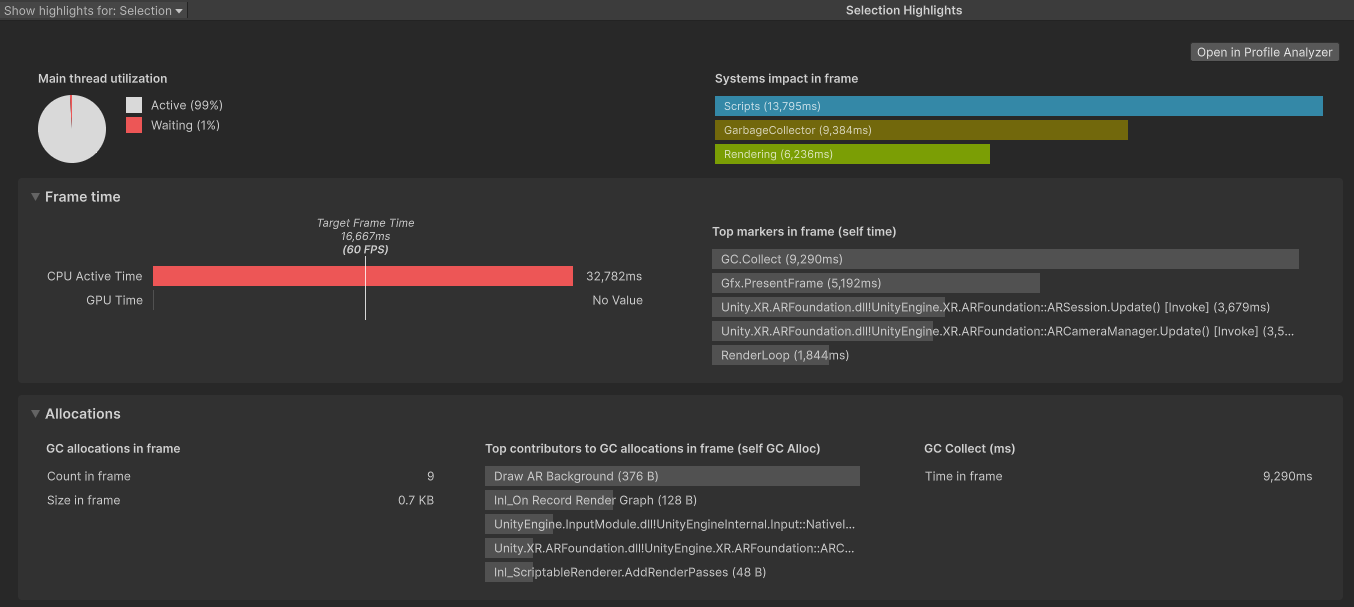
\includegraphics[width=0.7\textwidth]{images/app/HighLightsSelection.png} 
        \caption{Scheda \textit{Selection Highlights} dell'Unity Profiler.}
        \label{fig:highlightsselection}
\end{figure}
\begin{figure}[H]
        \centering
        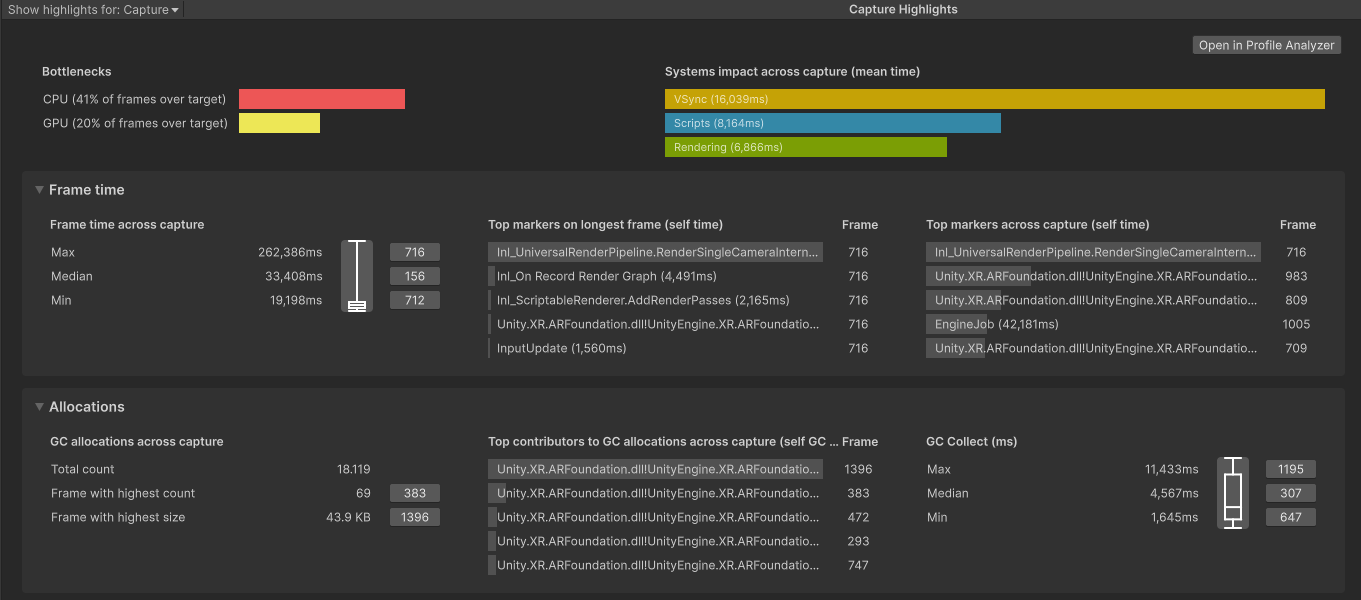
\includegraphics[width=0.7\textwidth]{images/app/HighLightsCapture.png} 
        \caption{Scheda \textit{Capture Highlights} dell'Unity Profiler.}
        \label{fig:highlightscapture}
\end{figure}

Le schede \textit{Selection Highlights} (SH, Figura~\ref{fig:highlightsselection}), relative al singolo frame selezionato, e \textit{Capture Highlights} (CH, Figura~\ref{fig:highlightscapture}), che offrono una panoramica statistica dell'intera sessione, riportano le seguenti metriche:

\begin{itemize}
\item \textbf{Utilizzo del Main Thread (SH):} attivo per il $99\%$ del tempo, con solo l'$1\%$ in attesa (\textit{Waiting}). Il dato è riferito al frame selezionato e potrebbe includere parte dei tempi di attesa di sincronizzazione (ad esempio il VSync).

\item \textbf{Impatto dei sistemi nel frame (SH):} \textit{Scripts} $13.795\text{ ms}$, \textit{GarbageCollector} $9.384\text{ ms}$, \textit{Rendering} $6.236\text{ ms}$.

\item \textbf{Colli di Bottiglia (CH):} il $41\%$ dei frame dell'intera cattura ha un tempo di CPU oltre il budget ($16.67\text{ ms}$; il frame time totale, invece, lo supera in ogni frame), mentre la GPU lo supera nel $20\%$ dei casi.

\item \textbf{Distribuzione del Frame Time (CH):} minimo $19.198\text{ ms}$ (frame $712$); mediana $33.408\text{ ms}$ (frame $156$), pari a circa $29.9\text{ FPS}$ e rappresentativa della frequenza tipica dell'applicazione; massimo $262.386\text{ ms}$, registrato al frame $716$, equivalente ad un blocco visibile di oltre un quarto di secondo. In questo frame il marker con il maggior tempo proprio (\textit{self time}, definito più sotto) è il rendering della camera della URP (\texttt{UniversalRender\allowbreak Pipeline.\allowbreak RenderSingle\allowbreak Camera\allowbreak Internal}) e non il Garbage Collector.

\item \textbf{Self Time (SH e CH):} misura il tempo netto speso in una funzione, escluse le sotto-funzioni chiamate. I principali contributi nel frame $808$ sono:
\begin{enumerate}
    \item \texttt{GC.Collect}: raccolta dei rifiuti sul Managed Heap, principale fattore di degrado temporaneo. Nel frame analizzato assorbe $9.290\text{ ms}$ ($\approx 28\%$ del tempo di frame), circa il doppio della mediana delle raccolte della cattura ($4.567\text{ ms}$); sull'intera sessione il massimo raggiunge $11.433\text{ ms}$.
    \item \texttt{Gfx.PresentFrame}: richiesta al sistema operativo e al display di mostrare il frame renderizzato. Assorbe $5.192\text{ ms}$, probabilmente legati alla sincronizzazione della presentazione (es. attesa del VSync).
    \item Routine AR Foundation (\texttt{ARSession} e \texttt{ARCameraManager}): $7.179\text{ ms}$ complessivi per l'elaborazione dei flussi video e dei sensori di tracciamento.
\end{enumerate}

\item \textbf{Mean Time (CH):} tempo medio occupato dai sistemi; i più rilevanti sono:
 \begin{itemize}
     \item \textbf{\texttt{VSync}} ($16.039\text{ ms}$): tecnologia che previene lo \textit{screen tearing} (la comparsa contemporanea di porzioni di fotogrammi diversi, visibile come interruzione orizzontale), obbligando la scheda grafica ad attendere il termine del ciclo di aggiornamento del display prima di inviare il fotogramma successivo. Nel profiler è tempo di attesa, non di lavoro.
     \item \textbf{\texttt{Scripts}} ($8.164\text{ ms}$): codice e logiche eseguite dalla CPU ad ogni frame. Un'elevata complessità ne aumenta la durata, ritardando il fotogramma successivo.
     \item \textbf{\texttt{Rendering}} ($6.866\text{ ms}$): fase in cui la CPU prepara i comandi grafici e la GPU elabora i dati geometrici e di illuminazione per generare i pixel dell'immagine; scene complesse, shader (programmi eseguiti dalla GPU per calcolare l'aspetto delle superfici) avanzati o risoluzioni elevate ne aumentano la latenza.
 \end{itemize}
In media, il lavoro effettivo (\textit{Scripts} più \textit{Rendering}, circa $15.0\text{ ms}$) rientra nel budget di $16.67\text{ ms}$, mentre la quota maggiore del frame time medio è attesa di VSync. Il frame time di circa $31\text{ ms}$ dipende quindi in larga parte dalla cadenza a $30\text{ FPS}$ e non solo dal carico computazionale; i picchi come \texttt{GC.Collect} possono invece spiegare i frame che superano il budget.
\end{itemize}

\subsection{Limiti della Sperimentazione}
I risultati vanno letti tenendo conto dei seguenti limiti:
\begin{itemize}
\item \textbf{Build di debug con Profiler collegato:} introducono un overhead aggiuntivo (il Profiler stesso occupa $36.9\text{ MB}$ di memoria); i valori assoluti sono quindi indicativi e, con ogni probabilità, peggiori rispetto a una build di rilascio.
\item \textbf{Singolo dispositivo:} i test sono stati eseguiti solo sul Motorola Edge 70, quindi i risultati non sono generalizzabili ad altri modelli o fasce di mercato.
\item \textbf{Frame selezionato:} l'analisi di dettaglio riguarda un singolo frame (il $808$), prossimo alla mediana, che non cattura la variabilità della sessione né il caso peggiore (frame $716$); per il comportamento complessivo si fa riferimento ai \textit{Capture Highlights}.
\item \textbf{Misura del tempo GPU:} il \textit{GPU Time} non è disponibile per il frame analizzato, quindi il carico grafico è stimato indirettamente.
\item \textbf{Limite alla frequenza di aggiornamento:} il tempo mediano di circa $33\text{ ms}$ potrebbe essere in parte determinato da un cap a $30\text{ FPS}$ (VSync, \texttt{Application.\allowbreak targetFrameRate} o cadenza del flusso della fotocamera) e non solo dal carico computazionale.
\end{itemize}












\chapter{Conclusioni}
Il confronto tra le due architetture non ha portato a un vincitore assoluto: nel corso del capitolo sono stati analizzati vantaggi e svantaggi di entrambi gli approcci, e la scelta dipende dagli obiettivi dello sviluppatore e dal tipo di applicazione da realizzare e distribuire.

AR Foundation è la soluzione più adatta quando il team di sviluppo è ridotto, l’applicazione deve essere distribuita su più piattaforme, i tempi di produzione devono essere rapidi e si accettano prestazioni comunque buone. Se invece sono prioritari il massimo delle prestazioni, l’accesso alle funzionalità più recenti e il pieno controllo dell’hardware, con un’integrazione completa con Android o iOS, la scelta più appropriata è l’uso diretto di ARCore o ARKit. \newline

 Inoltre, l'app sviluppata si presta a diversi ambiti applicativi: l'\textbf{arredamento e l'interior design}, per visualizzare mobili e complementi nello spazio domestico prima dell'acquisto; l'\textbf{e-commerce}, per anteprime in scala reale di prodotti; l'\textbf{architettura e l'edilizia}, per la presentazione di modelli e progetti sul sito; la \textbf{didattica e la divulgazione}, per esplorare modelli di oggetti, reperti o strutture anatomiche; e l'\textbf{intrattenimento}, ad esempio in giochi o esperienze interattive in realtà aumentata.
 
 L'analisi condotta con l'\textit{Unity Profiler} \textit{on-device} mostra che l'applicazione non raggiunge il target di $60\text{ FPS}$: il tempo mediano di frame è $33.408\text{ ms}$ (circa $30\text{ FPS}$), il minimo è $19.198\text{ ms}$ e si registrano picchi isolati fino a $262.386\text{ ms}$, dovuti al rendering della camera della URP. La CPU è il limite più frequente ($41\%$ dei frame oltre il budget, contro il $20\%$ della GPU), ma il lavoro effettivo medio (\textit{Scripts} e \textit{Rendering}, circa $15.0\text{ ms}$) rientra nel budget di $16.67\text{ ms}$, mentre la quota maggiore del frame time medio è attesa di VSync ($16.039\text{ ms}$): il valore mediano è quindi in larga parte riconducibile a una cadenza di $30\text{ FPS}$, da verificare, e non solo al carico computazionale. Il carico grafico, stimato indirettamente perché il \textit{GPU Time} non è disponibile per il frame analizzato, risulta contenuto ($42$ \textit{SetPass Calls}, $7$ chiamate di disegno in $4$ batch, circa $22\text{k}$ triangoli, $46.3\text{ MB}$ di texture), così come l'occupazione di memoria ($0.66\text{ GB}$ committed). Le criticità derivano dal costo del tracciamento AR, che nel frame analizzato assorbe quasi tutto il tempo degli \texttt{Update()} ($17.07$ su $18.33\text{ ms}$), e dalle allocazioni continue sul \textit{Managed Heap}, in gran parte originate da routine di AR Foundation e del rendering, che attivano il \textit{Garbage Collector}: questo assorbe fino a $11.433\text{ ms}$ e causa buona parte dei frame oltre il budget. 
 \newline
 
 Come sviluppi futuri si individuano diverse direzioni di ottimizzazione. In
primo luogo, la verifica del frame rate target e del cap a 30~FPS: il target
è la frequenza a cui l'applicazione dovrebbe girare e determina il tempo
massimo per produrre un frame (circa 33,3~ms a 30~FPS), per cui un frame time
vicino a tale valore non indica necessariamente una CPU satura, ma può
riflettere un'attesa imposta dal limite. In secondo luogo, l'identificazione,
tramite la vista \textit{Hierarchy} del Profiler ordinata per \textit{GC
Alloc}, dell'origine delle allocazioni, cioè delle richieste di memoria sul
\textit{Managed Heap}, l'area gestita automaticamente per il codice C\#; dove
queste dipendono dal codice dell'applicazione, possono essere ridotte
mediante \textit{caching} dei risultati di operazioni costose, ovvero salvarli in una variabile i riusarli, \textit{object
pooling}, ovvero riutilizzo di oggetti attivandoli e disattivandoli al posto di
\texttt{Instantiate} e \texttt{Destroy} e riuso di \textit{buffer}, ad
esempio la lista dei risultati dei raycast.
Inoltre si può valutare l'introduzione del Garbage Collector incrementale, che distribuisce su più frame la liberazione della memoria inutilizzata, riducendo i picchi di frame time a
fronte di un lieve overhead. 
Un ulteriore intervento riguarda la riduzione del costo del tracciamento AR, ossia dell'elaborazione con cui ARCore stima la posa del dispositivo e analizza l'ambiente, ad esempio disattivando le funzionalità non necessarie come il point cloud, la stima della luce o
l'occlusione, tenendo conto del compromesso con la robustezza dell'esperienza
d'uso. 
Infine, una nuova campagna di test con build di rilascio su più dispositivi permetterebbe di ottenere misure più vicine all'esperienza reale, poiché la build di debug con Profiler collegato introduce overhead, e di quantificare i miglioramenti confrontando, prima e dopo gli interventi, frametime e memoria utilizzata.


\bibliographystyle{unsrt}
\bibliography{main}
\end{document}
